\documentclass{article}
\usepackage[T2A]{fontenc}
\usepackage[utf8]{inputenc}
\usepackage[russian]{babel}
\usepackage{titling}
\usepackage{amsmath}
\usepackage{mathtools}
\usepackage{amsthm}
\usepackage{python}
% \usepackage{minted}
\usepackage{amssymb}
\usepackage{amsthm}
\usepackage{amsthm}
\usepackage{hyperref}
\usepackage{listings}
\usepackage{xcolor}

\usepackage{graphicx}
\graphicspath{ {./} }

\hypersetup{
    colorlinks,
    citecolor=black,
    filecolor=black,
    linkcolor=black,
    urlcolor=black
}
\usepackage{titlesec}
\usepackage[rightcaption]{sidecap}
\usepackage{wrapfig}
\titleformat*{\subsubsection}{\normalfont}

\makeatletter
\renewcommand*\env@matrix[1][*\c@MaxMatrixCols c]{%
  \hskip -\arraycolsep
  \let\@ifnextchar\new@ifnextchar
  \array{#1}}
\makeatother


\setlength{\droptitle}{-3.5cm}
\setlength{\parindent}{0cm}
\newcommand{\squad}{\hspace{0.5em}}
\renewcommand{\arraystretch}{1.5}

\newtheorem{theorem}{Теорема}
\newtheorem{lemma}{Лемма}
% \renewcommand{\sectionbreak}{}

\author{Макаров Максим}
\title{Весенний коллоквиум по дискретной математике}
\date{}
\usepackage
[
        a4paper,
        left=2cm,
        right=2cm,
        top=3cm,
        bottom=4cm
]
{geometry}

\begin{document}
\begin{samepage}
\maketitle
\tableofcontents{}
\end{samepage}
\section{Список определений}
\begin{samepage}
\subsection{Деление целых чисел с остатком.}
Говорят, что целое число $a$ делится на целое число $b$ ($a$ кратно $b$), если $a = bk$ для некоторого целого числа $k$. Разделить целое $a$ на целое положительное $b$ означает найти такое целое $q$ (частное) и такое целое $r$ (остаток), что
\[
a = b \cdot q + r;
\quad
0 \leqslant r < b
\]


\subsection{Сравнения по модулю. Основные свойства.}
Если два числа $a$ и $b$ дают одинаковые остатки при делении на положительное число $N$, то говорят, что они \textit{сравнимы} по модулю $N$, и пишут $a \equiv b \mod{N}$. Сравнение по модулю -- \textit{отношение эквивалентности} на множестве целых чисел.
% \newline
% Основные свойства:
% \begin{enumerate}
%     \item $a + b = b + a$ (коммутативность сложения)
%     \item $a + (b + c) = (a + b) + c$ (ассоциативность сложения)
%     \item $ab = ba$ (коммутативность умножения)
%     \item $a(bc) = (ab)c$ (ассоциативность умножения)
%     \item $a(b + c) = ab + ac$ (дистрибутивность)
%     \item $0+a = a$
%     \item $1 \cdot a = a$
%     \item $0 \cdot a = 0$
% \end{enumerate}
\subsection{Арифметика остатков (вычетов). Обратимые остатки (вычеты).} 
Основные свойства:
\begin{enumerate}
    \item $a + b \equiv b + a$ (коммутативность сложения)
    \item $a + (b + c) \equiv (a + b) + c$ (ассоциативность сложения)
    \item $ab \equiv ba$ (коммутативность умножения)
    \item $a(bc) \equiv (ab)c$ (ассоциативность умножения)
    \item $a(b + c) \equiv ab + ac$ (дистрибутивность)
    \item $0+a \equiv a$
    \item $1 \cdot a \equiv a$
    \item $0 \cdot a \equiv 0$
\end{enumerate}
Остаток (вычет) по модулю $N$ называется \textit{обратимым}, если в произведении с каким-то другим остатком он дает 1. Другими словами, $a$ обратим, если уравнение $ax = 1$  имеет решение.
\end{samepage}
\subsection{Малая теорема Ферма.}
Если $p$ -- простое число и $a$ не делится на $p$, то $a^{p-1}$ сравнимо с $1$ по модулю $p$, то есть $a^{p-1} \equiv 1 \mod{p}$.


\subsection{Функция Эйлера. Теорема Эйлера.}
\textbf{Определение функции Эйлера} \newline
Пусть $N > 1$ -- произвольное целое число, тогда функцию $\varphi(N)$, равную количеству остатков среди $0,1,...,N-1$, взаимно простых с $N$, называют функцией Эйлера.
\newline
Основные свойства функции Эйлера:
\begin{itemize}
    \item $\varphi(p^n) = p^n(1-1/p) = p^{n-1}(p - 1)$ для простого $p$
    \item $\varphi(uv) = \varphi(u)\varphi(v)$, если $u$ и $v$ взаимно просты
\end{itemize}
\textbf{Теорема Эйлера} \newline
Если $a$ и $m$ взаимно просты, то $a^{\varphi(m)} \equiv 1 \mod{m}$, где $\varphi(m)$ -- функция Эйлера.

\subsection{Наибольший общий делитель. Алгоритм Евклида.}
\[
\text{НОД}(a, b) := max (\{ x \> | \> a \text{ кратно } x \} \cap \{ x \> | \> b \text{ кратно } x \})
\]

\begin{lstlisting}[language=Python]
def gcd(a, b):
    if a*b == 0:
        return a + b
    if a > b:
        return gcd(a % b, b)
    return gcd(a, b % a)
\end{lstlisting}




\subsection{\textcolor{orange}{(UNCHECKED)} Расширенный алгоритм Евклида нахождения решения линейного диофантова уравнения.}
\textit{Линейные диофантовы уравнения} -- уравнения вида
\[
a_1x_1 + a_2x_2 + ... + a_nx_n = d,
\] где $a_1,...,a_n$ -- целые числа, а переменные $x_i$ принимают целые значения.
\newline
\newline
Расширенный алгоритм Евклида позволяет находить решения линейного диофантова уравнения 
\[
ax + by = c \text{, где } c = \text{НОД}(a,b).
\]
\begin{lstlisting}[language=Python]
def gcd_expanded(a, b):
    x, x2, y, y2 = 1, 0, 0, 1
    while (a*x + b*y)*(a*x2 + b*y2) > 0:
        if (a*x + b*y) > (a*x2 + b*y2):
            x -= x2
            y -= y2
        else:
            x2 -= x
            y2 -= y
    return (x, y)
\end{lstlisting}




\subsection{Простые числа, формулировка основной теоремы арифметики.}
Целое число $p > 1$ называется \textit{простым}, если оно не разлагается в произведение меньших чисел (то есть не имеет положительных делителей, кроме 1 и $p$).
\newline
\newline
Всякое целое положительное число, большее 1, разлагается на простые множители, причем единственным образом: любые два разложения отличаются только перестановкой сомножителей.



\subsection{Равномощные множества.}
Множество $A$ называется равномощным множеству $B$, если существует биекция из множества $A$ в множество $B$.
\newline
Свойства равномощности:
\begin{itemize}
    \item \textit{Отношение равномощности симметрично}: если $A$ равномощно множеству $B$, то $B$ равномощно $A$. В самом деле, как мы уже обсуждали, ко всякой биекции есть обратная функция — тоже биекция.
    \item \textit{Отношение равномощности рефлексивно}: каждое множество равномощно само- му себе. В самом деле, тождественная функция, которая отображает каждый элемент какого-то множества $A$ в себя, является биекцией между $A$ и $A$.
    \item \textit{Отношение равномощности транзитивно}: если $A$ равномощно $B$ и $B$ равномощно $C$, то $A$ равномощно $C$, так как композиция биекций -- биекция.
\end{itemize}
Таким образом, отношение равномощности является \textit{отношением эквивалентности}.


\subsection{Счётные множества.}
Счётные множества -- это множества равномощные множеству натуральных чисел $\mathbb{N}$.
\newline
Основные свойства счётных множеств:
\begin{itemize}
    \item \textit{Объединение двух счётных множеств счётно.}
    \item \textit{Всякое подмножество счётного множества конечно или счётно.}
    \item \textit{Всякое бесконечное множество содержит счётное подмножество.}
    \item \textit{Множество рациональных чисел $\mathbb{Q}$ счетно.}
    \item \textit{Объединение конечного или счётного числа конечных или счётных множеств конечно или счётно.}
    \item \textit{Декартово произведение двух счётных множеств $A$ × $B$ cчётно.}
\end{itemize}


\subsection{Множества мощности континуум.}
Множество $A$ имеет мощность континуум, если $A$ равномощно $\mathbb{R}$.
\newline
Основные свойства:
\begin{itemize}
    \item  $[0,1] \sim \mathbb{R}$
    \item  $(0,1) \sim \mathbb{R}$
    \item  $\mathbb{R} \times \mathbb{R} \sim \mathbb{R}$
    \item Множество бесконечных последовательностей нулей и единиц несчётно.
    \item Отрезок $[0, 1]$ равномощен множеству бесконечных последовательностей из нулей и единиц.
\end{itemize}

\subsection{Основные определения элементарной теории вероятностей: исходы, события, вероятность события.}
\textit{Вероятностным пространством} называется конечное множество $U$, которое состоит из \textit{возможных исходов} и на котором задана функция $Pr : U \to [0, 1]$, такая что $\sum_{ x \in U} Pr(x) = 1$.
\newline
\newline
Функция $Pr$ называется \textit{вероятностным распределением}, а число $Pr(x)$ называется \textit{вероятностью исхода} $x \in U$.
\newline
\newline
\textit{Событием} называется произвольное подмножество $A \subset U$, состоящее из \textit{благоприятных исходов}.
\newline
\newline
\textit{Вероятностью события} $A$ называется число $Pr[A] = \sum_{x \in A} Pr(x)$.
\newline
\newline
В \textit{модели с равновозможными исходами} функция $Pr$ задается формулой $Pr[x] = 1/|U|$ для всякого $x \in U$ (такое распределение называют также \textit{равномерным}). Тогда вероятность события $A$ равна $Pr[A] = |A|/|U|$.



\subsection{Формулировка формулы включений и исключений для вероятностей.}
Если $A, B \subset U$, то 
\(
Pr[A \cup B] = Pr[A] + Pr[B] - Pr[A \cap B].
\)
В частности, \(
Pr[A \cup B] \leqslant Pr[A] + Pr[B]
\) и, если $Pr[A \cap B] = 0$, то \(
Pr[A \cup B]=Pr[A]+Pr[B].
\)
\newline
\newline
Для любых $A_1, ... , A_n \subset U$ верно
\[
Pr [
\bigcup_{i=1}^n A_i
] \leqslant
\sum_{i=1}^n Pr[A_i],
\]
а если множества $A_i$ попарно не пересекаются, то неравенство обращается в равенство (это называется аддитивностью вероятностей для попарно несовместных событий).
\newline
\newline
В \textit{равновозможной модели} для произвольных множеств $A_1,...,A_n \subset U$ верно
\[
Pr[A_1 \cup A_2 \cup ... \cup A_n] = \sum_i Pr[A_i] - \sum_{i<j} Pr[A_i \cap A_j] + ... = \sum_{\varnothing \neq I \subset \{1,2,...,n\}} (-1)^{|I| + 1} Pr \left[ \bigcap_{i \in I} A_i \right].
\]


\subsection{Условная вероятность.}
\textit{Условной вероятностью события $A$ при условии $B$} называется число
\[
Pr[A | B] = \frac{Pr[A \cap B]}{Pr[B]}.
\]
\begin{lemma}
\normalfont{(формула Байеса).} Если вероятность событий $A$ и $B$ положительна, то
\[
Pr[A | B] = Pr[A] \cdot \frac{Pr[B | A]}{Pr[B]}.
\]
\end{lemma}


\subsection{Независимые события. Основные свойства независимых событий.}
События $A$ и $B$ называются независимыми, если $Pr[A | B] = Pr[A]$ при $Pr[B] > 0$. 
\newline
Основные свойства независимых событий:
\begin{itemize}
    \item Если события $A$ и $B$ независимы, то события $A$ и $\overline{B}$, $\overline{A}$ и $B$, $\overline{A}$ и $\overline{B}$ также независимы.
    \item Если события $A$ и $B$ независимы, то $Pr[AB] = Pr[A] \cdot Pr[B]$.
\end{itemize}


\subsection{Формула полной вероятности.}
Пусть $B_1,...,B_n$ -- разбиение вероятностного пространства U, то есть $U = B_1 \cup ... \cup B_n$, где $B_i \cap B_j = \varnothing$ при $i \neq j$. Пусть также $Pr[B_i] > 0$ для всякого $i$. Тогда для всякого события $A \subset U$
\[
Pr[A] = \sum_{i=1}^n Pr[A | B_i] \cdot Pr[B_i].
\]




\subsection{Случайная величина и математическое ожидание. Линейность математического ожидания.}
\textit{Случайная величина} -- это числовая функция на вероятностном пространстве, то есть функция вида $f : U \to \mathbb{R}$.
\newline
\newline
\textit{Математическим ожиданием} случайной величины $f : U \to \mathbb{R}$ называется число
\[
E[f] = \sum_{u \in U} f(u)Pr(u)
\]
\newline
Пусть $f : U \to \mathbb{R}$ и $g : U \to \mathbb{R}$ -- две случайные величины на одном и том же вероятностном пространстве. Тогда
\[
E[f + g] = E[f] + E[g]. 
\]



\subsection{Формулировка неравенства Маркова.}
Пусть $f$ — случайная величина, принимающая только неотрицательные значения. Тогда для всякого $\alpha > 0$ верно
\[
Pr[f \geqslant \alpha] \leqslant \frac{E[f]}{\alpha}.
\]

\subsection{Определение схемы в некотором функциональном базисе. Представление схем графами.}
\begin{wrapfigure}{r}{0.4\textwidth}
    \centering
    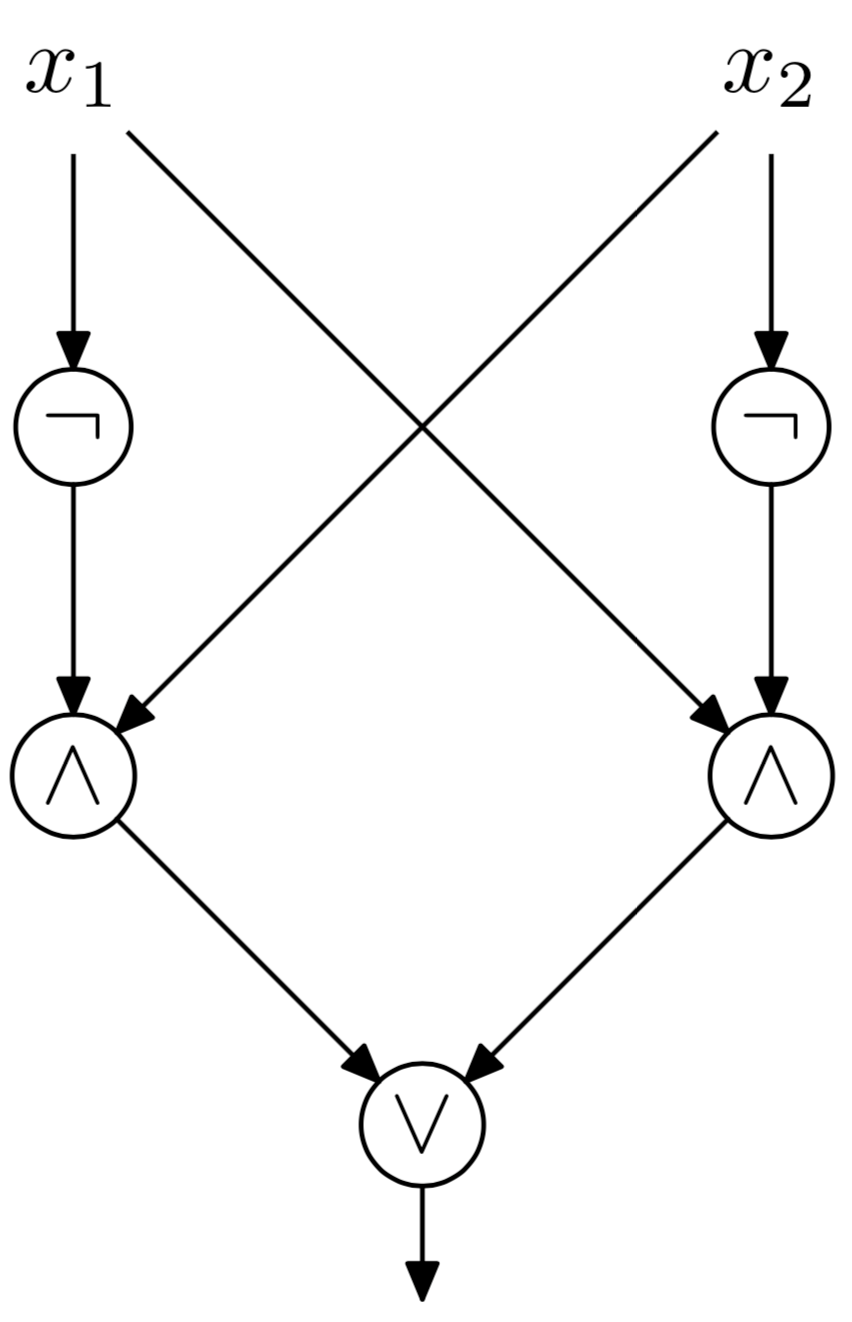
\includegraphics[width=0.25\textwidth]{graph}
    \caption{Схема для функции $x_1 \oplus x_2$}
\end{wrapfigure}

\textit{Булевой схемой} от переменных $x_1, ..., x_n$ называется последовательность булевых функций $g_1,...,g_s$, в которой всякая $g_i$ получается из предыдущих функций последовательности и переменных применением одной из логических операций: отрицание, конъюнкция и дизъюнкция. Другими словами, для всякого $i$ имеет место одно из равенств
\[
g_i = g_j \wedge g_k \> (j, k < i),
\quad
g_i = g_j \vee g_k \> (j,k < i),
\]
\[
g_i = g_j \wedge x_k \> (j < i),
\quad
g_i = g_j \vee x_k \> (j < i),
\]
\[
g_i = x_j \wedge x_k,
\quad
g_i = x_j \vee x_k,
\]
\[
g_i = \neg g_j \> (j < i),
\quad
g_i = \neg x_k.
\]
Имея в виду эти связи между элементами последовательности (схемы), будем также называть элементы схемы \textit{присваиваниями}.
\newpage

\subsection{Полный базис. Примеры полных и неполных базисов.}
\textit{Полный логический базис} -- это такая система логических функций, с помощью которых можно записать любую, сколь угодно сложную функцию. 
\newline
Примеры полных логических базисов:
\begin{itemize}
    \item $\{\wedge, \vee, \neg\}$
    \item $\{\vee, \neg\}$
    \item $\{\wedge, \neg\}$
    \item $\{x \downarrow y\}$ (стрелка Пирса)
    \item $\{x | y\}$ (штрих Шеффера)
    \item $\{\wedge, \oplus, 1 \}$ (базис Жегалкина)
\end{itemize}
Примеры неполных логических базисов:
\begin{itemize}
    \item $\{\wedge, \vee\}$
    \item $\{\oplus \}$
\end{itemize}




\subsection{Полином Жегалкина (в стандартном виде).}
Выражения вида
\[
P(x_1,...,x_n) = a_0 \oplus a_1x_1 \oplus a_2x_2 \oplus ... \oplus a_nx_n \oplus a_{12}x_1x_2 \oplus a_{13}x_1x_3 \oplus ... \oplus a_{1...n}x_1...x_n,
\quad
a_0,...,a_{1...n} \in \{0,1\}.
\]
называются \textit{полиномами Жегалкина}.
\newline
\newline
Всякая булева функция представима в виде полинома Жегалкина и притом единственным образом.


\subsection{Схемная сложность функции (размер схемы).}
\textit{Схемная сложность} булева отображения $f : \{0, 1\}^n \to \{0, 1\}^m$ (в частности, булевой функции) — это наименьший размер схемы, вычисляющей это отображение.
\newline
\newline
Всякую функцию $f : \{0, 1\}^n \to \{0, 1\}$ можно вычислить схемой размера не больше $O(n2^n)$.




\newpage


\section{\textcolor{red}{(TODO)} Примерные задачи на понимание материала курса}
 
\subsection*{\normalsize{\normalfont{
Привидите пример таких целых чисел $a, b, c$, что НОД$(ab,c) \neq $НОД$(a,c) \cdot $НОД(b,c).
}}} 

\newpage




\section{Вопросы на знание доказательств}
\subsection{Сравнение $ax \equiv 1 \mod{N}$ имеет решение тогда и только тогда, когда $\text{\normalfont{НОД}}(a, N) = 1$.}
\begin{theorem}
Обратимыми по модулю $N$ являются те и только те остатки, которые взаимно просты с $N$.
\end{theorem}
Например, по модулю 10 отпадают все чётные числа (у которых общий делитель 2), а также число 5 (общий делитель 5), остаются как раз 1, 3, 7, 9.
\newline
В частности, если $N$ простое (не разлагается в произведение меньших чисел), то общим делителем могут быть только 1 и $N$, так что все остатки, кроме нуля, взаимно просты с $N$ и обратимы. Для простого модуля действуют все обычные правила сложения и умножения (как в обычной алгебре), и делить можно на всё кроме нуля. (Математики выражают это словами: вычеты по простому модулю $p$ образуют поле.)
\newline
Прежде чем доказывать эту теорему, представим себе наглядно, что означает обратимость остатка $a$. Для этого вспомним, что остатки по модулю $N$ можно расположить на круговом шоссе длины $N$, как автобусные остановки. Запустим маршрут автобуса, которые делает остановки каждые $a$ километров: у него первая остановка будет в $a$, вторая в $a + a = 2a$, третья в $3a$ (всё по модулю $N$ , естественно). Обратимость означает, что таким странным способом все остановки будут обслужены (в строке таблицы умножения встретятся все остатки).
\newline
Вот две картинки, показывающие, что по модулю 10 остаток 3 будет обратимым, $a$ остаток 4 нет:
\begin{center}
    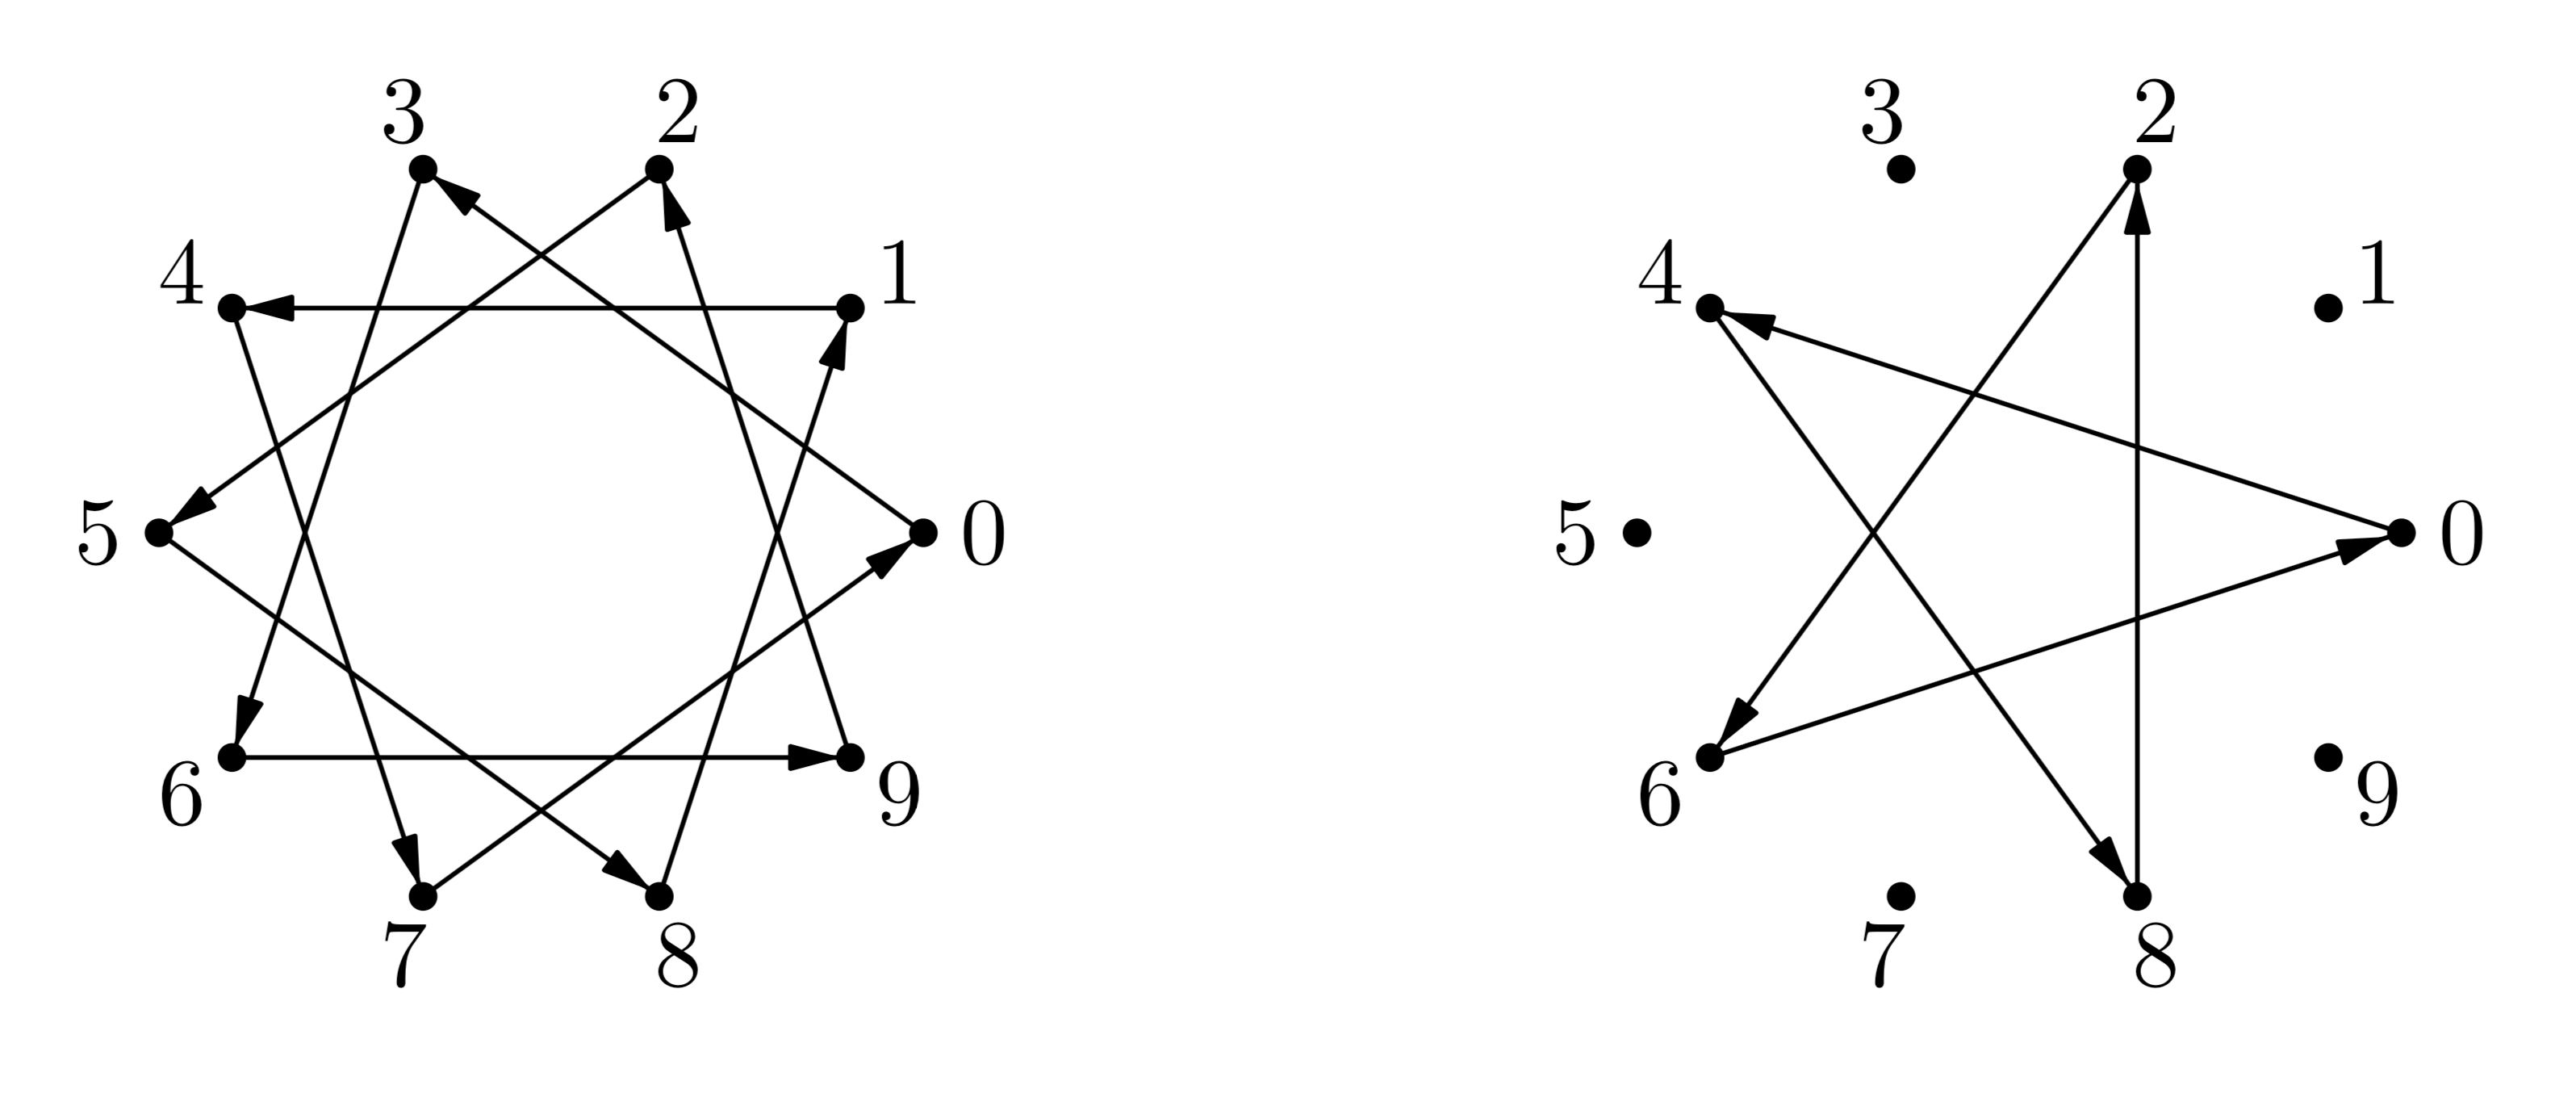
\includegraphics[width=0.6\textwidth]{buses}
\end{center}
в первом случае мы проходим все остановки, а во втором не все (только чётные).
\newline
Кстати, из этой картинки хорошо видно, что если элемент обратим (мы попадаем в соседнюю остановку), то деление всегда возможно (мы попадём во все остановки). В самом деле, если через k шагов мы попали в соседнюю, то ещё через $k$ мы попадём
в следующую и так далее, пройдя через все остановки.
\newline
Теперь легко доказать простую часть утверждения: если $N$ и шаг a имеют общий
делитель $d$, то элемент a необратим (мы не попадём в соседнюю остановку). В самом деле, будем отмечать остановки через $d, 2d, 3d$ и так далее от начальной. Поскольку $N$ делится на $d$, то мы дойдём до $N$-й (то есть начальной) остановки, пройдя весь круг. Если a кратно $d$, то $a$-автобус будет останавливаться только в выделенных остановках, и в соседнюю никогда не попадёт.
\newline
Осталось доказать сложную часть утверждения: если $N$ и шаг $a$ не имеют общих делителей, то все остановки будут обслужены. Тут полезно вспомнить о перестановках и отвечающих им ориентированных графах.
\newline
В нашем случае вершины графа расположены по кругу, как вершины правильного $N$-угольника. Стрелки (рёбра графа) соответствуют движению автобуса, проезжающего $a$ перегонов до следующей остановки. Другими словами, из вершины $x$ (остатка по модулю $N$ ) стрелка ведёт в вершину $x + a$. По построению из каждой
вершины выходит только одна стрелка, и входит тоже только одна, из вершины $x-a$ (однозначность вычитания). Нам надо доказать, что если $a$ взаимно просто с $N$, то есть только один цикл, включающий все вершины.
\newline
Пусть цикл, начатый из вершины 0, включает только часть вершин. Посмотрим, в какие вершины он попадает. Пусть ближайшая из них (по кругу) имеет номер $d$.
Ясно, что построение цикла можно начать с любой вершины (круг везде одинаков), поэтому если мы начнём с $d$, то следующая обслуженная вершина будет $2d$. Значит, в цикл входят вершины 0, потом (по кругу) $d$, потом $2d$ и так далее, пока мы не вернёмся обратно в начальную вершину 0. В результате мы пройдём полный круг в $N$ вершин, двигаясь шагами по $d$, поэтому $N$ кратно $d$. С другой стороны, вершина $a$ обслужена (на первой же остановке автобуса), поэтому и $a$ тоже кратно $d$. Получается, что $d$ — общий делитель $N$ и $a$. А мы предположили, что они взаимно просты, то есть $d$ = 1, что означает, что все вершины (все остатки по модулю N) попадают в один цикл.



\subsection{Малая теорема Ферма.}
\begin{lemma}
Для любого простого числа $p$ и целого числа $k$, не кратного $p$, произведения $k$ и чисел $1,2,3,...,p-1$ при делении по модулю на $p$ в остатке дают те же самые числа $1,2,3,...,p-1$, возможно, записанные в некотором другом порядке.
\begin{proof}
Произведение $k$ и любого из чисел $1,2,3,...,p-1$ не кратно $p$, следовательно, в остатке не может получиться 0. Все остатки разные. Докажем последнее утверждение от противного. Пусть два произведения $ak$ и $bk$ дают при делении на $p$ одинаковые остатки, тогда разность $ak - bk = (a - b)k$ кратна $p$, что невозможно, поскольку $a - b$ не кратно $p$. Всего существует $p-1$ различных остатков от деления на $p$.
\end{proof}
\end{lemma}
\begin{theorem}
Если $p$ -- простое число и $a$ не делится на $p$, то $a^{p-1}$ сравнимо с $1$ по модулю $p$, то есть $a^{p-1} \equiv 1 \mod{p}$.
\begin{proof}
Поскольку согласно вышеприведенной лемме остатки от деления чисел $a, 2a, 3a, ..., (p-1)a$ -- это с точностью до перестановки числа $1,2,3,...,p-1$, то $a \cdot 2a \cdot 3a \cdot ... \cdot (p-1)a \equiv 1 \cdot 2 \cdot 3 \cdot ... \cdot (p-1) \mod{p}$. Отсюда $a^{p-1}(p-1)! \equiv (p-1)! \mod{p}$. Последнее соотношение можно сократить на $(p-1)!$, поскольку все сомножители являются числами, взаимно простыми с основанием $p$, и в результате получаем требуемое утверждение $a^{p-1} \equiv 1 \mod{p}$
\end{proof}
\end{theorem}
\subsection{Теорема Эйлера.}
\begin{theorem}
Если $a$ и $m$ взаимно просты, то $a^{\varphi(m)} \equiv 1 \mod{m}$, где $\varphi(m)$ -- функция Эйлера.
\begin{proof}
Пусть $x_1,...,x_{\varphi(m)}$ -- все различные натуральные числа, меньшие $m$ и взаимно простые с ним. Рассмотрим все возможные произведения $x_ia$ для всех $i$ от 1 до $\varphi(m)$.
Поскольку $a$ взаимно просто с $m$ и $x_i$ взаимно просто с  $m$, то и $x_ia$ также взаимно просто с $m$, то есть $x_ia \equiv x_j \mod{m}$ для некоторого $j$.
Отметим, что все остатки $x_ia$ при делении на $m$ различны. Действительно, пусть это не так, тогда существуют такие $i_1 \neq i_2$, что
\[
x_{i_1}a \equiv x_{i_2}a \mod{m}
\Leftrightarrow
(x_{i_1} - x_{i_2})a \equiv 0 \mod{m}.
\]
Так как $a$ взаимно просто с $m$, то последнее равенство равносильно тому, что
\[
x_{i_1} - x_{i_2} \equiv 0 \mod{m}
\Leftrightarrow
x_{i_1} \equiv x_{i_2} \mod{m}.
\]
Это противоречит тому, что числа $x_1,...,x_{\varphi(m)}$ попарно различны по модулю $m$.
Перемножим все сравнения вида $x_ia \equiv x_j \mod{m}$. Получим:
\[
x_1...x_{\varphi (m)}a^{\varphi (m)} \equiv x_1...x_{\varphi (m)} \mod{m}
\Leftrightarrow
x_1...x_{\varphi (m)}(a^{\varphi (m)} - 1) \equiv 0 \mod{m}.
\]
Так как число $x_1...x_{\varphi (m)}$ взаимно просто с $m$, то последнее сравнение равносильно тому, что
\[
a^{\varphi (m)} - 1 \equiv 0 \mod{m}
\Leftrightarrow
a^{\varphi (m)} \equiv 1 \mod{m}.
\]
\end{proof}
\end{theorem}
\subsection{Корректность алгоритма Евклида и расширенного алгоритма Евклида.}
\textbf{Алгоритм Евклида}
\newline
\newline
Давайте сначала посмотрим на этот алгоритм в том виде, как это было у Евклида в его учебнике геометрии (<<Начала>>). Пусть нам надо найти общую меру двух отрезков, то есть третий отрезок, который укладывается целое число раз в первом и во втором. (Другими словами, мы хотим найти меру длины, при которой длины обоих данных нам отрезков будут целыми числами).
\newline
Евклид предлагает делать это так: будем откладывать меньший отрезок $m$ внутри большего $M$. Если нам повезёт и он уложится целое число раз, то меньший отрезок $m$ и будет общей мерой. Если нет, то он уложится сколько-то раз и что-то (уже меньшее $m$) останется. Обозначим этот остаток за $r$. Теперь повторим эту процедуру с отрезками $m$ и $r$, укладывая меньший из них (то есть $r$) в большем. Снова либо он уложится без остатка, либо получится остаток $r'$, меньший $r$, и мы применяем алгоритм к $r$ и $r'$, и так далее. Алгоритм заканчивает свою работу, когда и если меньший отрезок укладывается в большем без остатка.
\begin{center}
    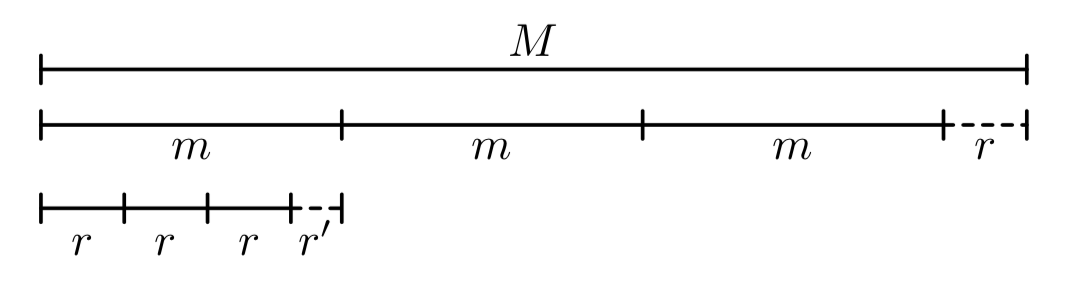
\includegraphics[width=0.5\textwidth]{evklid1}
\end{center}
Другой способ представить ту же самую процедуру получается, если считать отрезки сторонами прямоугольников: сначала есть прямоугольник $M \times m$, от которого отрезают квадраты $m \times m$, пока это возможно. Когда останется прямоугольник $r \times m$, в котором $r < m$, от него отрезают квадраты $r \times r$, остаётся прямоугольник $r \times r'$ с $r' < r$. Можно считать, что у нас есть автомат, который отрезает от прямоугольника квадрат со стороной, равной меньшей стороне прямоугольника (он сам разбирается, какая сторона меньше). Мы кромсаем прямоугольник на квадратные части, засовывая остаток снова и снова в этот автомат.
\begin{center}
    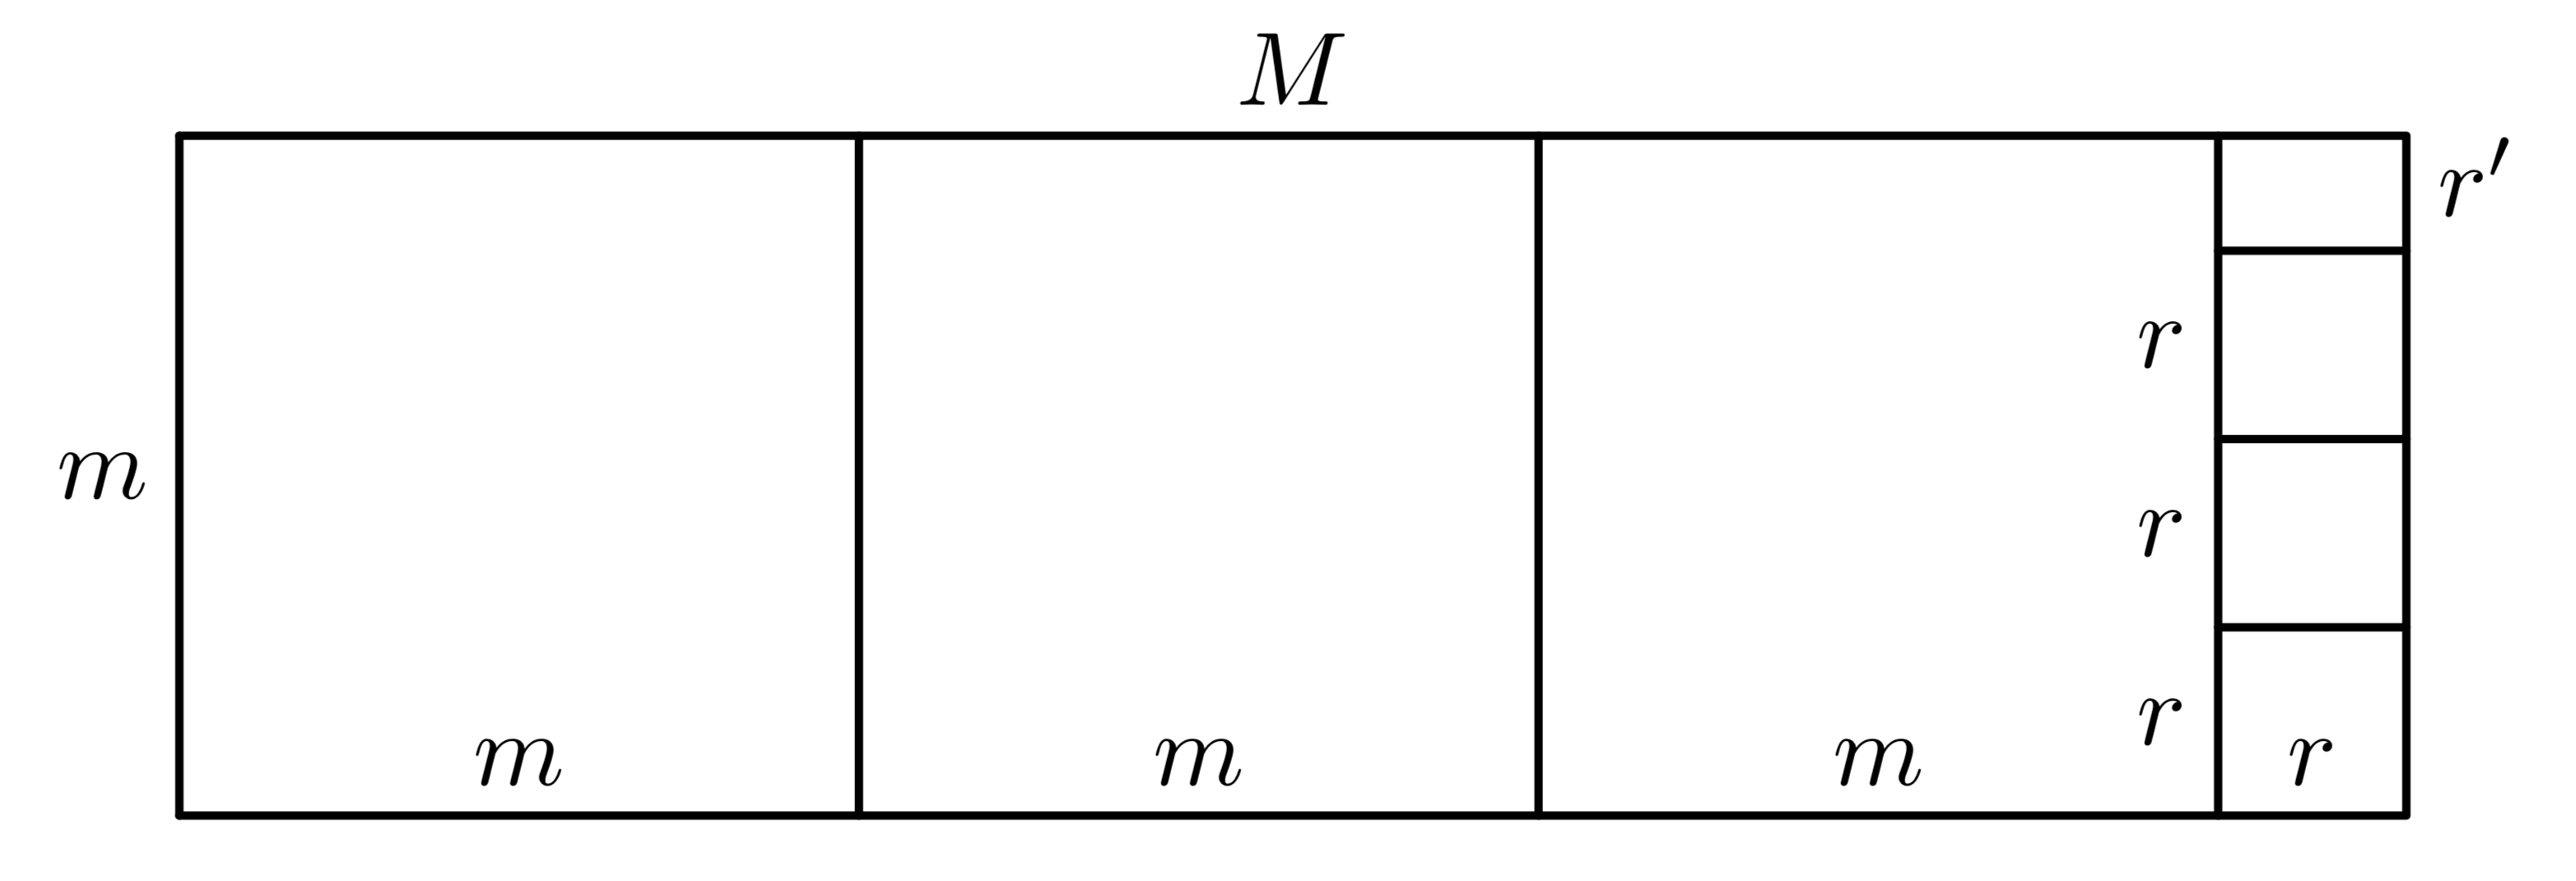
\includegraphics[width=0.5\textwidth]{evklid2}
\end{center}
По существу это, конечно, тот же самый процесс, может быть, в немного более наглядной форме.
\newline
Основное свойство алгоритма Евклида теперь можно сформулировать так:
\begin{theorem}
Если исходные отрезки имеют общую меру, то алгоритм заканчивает работу и последний отрезок (тот, что уложится целое число раз) будет наибольшей их общей мерой. Если же исходные отрезки не имеют общей меры, то алгоритм никогда не остановится.
\begin{proof}
\textbf{(1) } Если исходные отрезки имеют общую меру $d$, примем её за единицу измерения. Тогда оба наших отрезка имеют целую длину, и мы делим одно целое число $(M)$ на другое $(m)$ с остатком $r$, потом делим $m$ на $r$ с остатком $r'$ и так дальше, при этом $m > r > r' > ...$ (остаток меньше делителя) и все они целые, так что бесконечно это продолжаться не может. В терминах прямоугольников: нарисуем всё по клеточкам на клетчатой бумаге с шагом $d$, тогда и все разрезы пройдут по клеточкам, и возможных мест разреза конечное число.
\newline
\newline
\textbf{(2) } Теперь покажем, что если алгоритм заканчивает работу, то последний отрезок будет общей мерой. В самом деле, если принять его за единицу измерения, то предыдущий отрезок будет целым числом (ведь последний укладывается целое число раз), перед ним тоже будет целый отрезок (равный сумме нескольких целых чисел) и пр. В терминах квадратов: если принять самый маленький квадрат при разрезании за клетку на клетчатой бумаге, то все большие квадраты и составленные их них прямоугольники пойдут по линиям сетки, и их стороны будет целыми, то есть сторона маленького квадрата будет общей мерой. (Отсюда уже следует последнее утверждение: если общей меры нет, то алгоритм не заканчивает работу.)
\newline
\newline
\textbf{(3) } Осталось показать, что последний отрезок будет наибольшей общей мерой. Более того, он даже будет кратен любой другой общей мере $d$. Почему? Приняв $d$ за единицу измерения, мы видим, что оба наших отрезка имеют целую длину, и все последующие отрезки будут целыми. Значит, ответ алгоритма Евклида тоже целый (кратен $d$), как мы и утверждали.
\end{proof}
\end{theorem}
% \newline
% \newline
\textbf{Алгоритм Евклида и диофантовы уравнения}
\newline
\newline
Мы можем найти $d = \text{НОД}(a, b)$, разрезая на квадраты прямоугольник $a \times b$, это будет сторона наименьшего из квадратов. Ключевое наблюдение: \textit{все стороны квадратов, появляющиеся в ходе алгоритма, представляются в виде $ax + by$ с некоторыми целыми $x$ и $y$.} Как говорят, они являются «целочисленными линейными комбинациями» $a$ и $b$. Это же относится и к последнему отрезку, то есть $d$, и мы получаем искомое решение.
\newline
Почему они будут целочисленными линейными комбинациями? Пусть мы сначала делим $a$ на $b$ с остатком $r$, тогда $a = bq+r$, и $r = a-bq$ представлен такой комбинацией. Теперь мы делим $b$ на $r$, получаем остаток $r'$, то есть $b = q'r + r'$, и $r' = b - q'r$ есть целочисленная комбинация $b$ и $r$. Вспомним, что само $r$ есть комбинация $a$ и $b$, получится
\[
r' = b - q'r = b - q'(a-bq) = b - q'a + q'bq = (qq' + 1)b - q'a,
\]
то есть $r'$ тоже есть целочисленная комбинация $a$ и $b$, и так далее.









\subsection{Основная теорема арифметики.}
\begin{theorem}
Всякое целое положительное число, большее 1, разлагается на простые множители, причём единственным образом: любые два разложения отличаются только перестановкой сомножителей.
\begin{proof}
\textit{Существование разложения} совсем просто. Если данное число $N$ простое, то получилось разложение из одного сомножителя. Если нет, то $N = ab$ для каких-то меньших $a$, $b$. Если $a$ и $b$ простые, то хорошо, если нет, то разложим их в произведение меньших и так далее до тех пор, пока дальше уже ничего не раскладывается, поскольку числа простые. (Формально говоря, мы рассуждаем по индукции и считаем, что для меньших чисел $a$ и $b$ существование разложения уже известно.)
\newline
\textit{Единственность разложения}. Пусть некоторое число $N$ имеет два разложения
\[
N = p_1 \cdot p_2 \cdot ... \cdot p_n = q_1 \cdot q_2 \cdot ... \cdot q_m
\]
(они могут отличаться и числом сомножителей, $m$ не обязано равняться $n$). Мы хотим получить противоречие. Сократим на общие сомножители (если они есть). Если сократится не всё, то получим два разложения одного числа, не имеющих общих сомножителей
\[
p_1 \cdot p_2 \cdot ... \cdot p_n = q_1 \cdot q_2 \cdot ... \cdot q_m.
\]
Как говорят, <<без ограничения общности>> можно предположить, что общих сомножителей нет (сократив на них, если есть).
\newline
В чём тут противоречие? С одной стороны, левая часть делится на $p_1$ (можно было бы взять любой другой $p_i$, если там несколько сомножителей). А правая часть равна произведению чисел, ни одно из которых не делится на $p_1$: они ведь простые и $p_1$ среди них по предположению нет. Осталось доказать, что такого не бывает, то есть доказать следующую лемму.
\begin{lemma}
Если $p$ — простое число, то произведение чисел, не делящихся на $p$, не может делиться на $p$.
\end{lemma}
По существу мы уже это доказали: в терминах вычетов по модулю $p$ нужно доказать, что произведение ненулевых вычетов не равно нулю. А мы знаем, что если $a \neq 0 \mod{p}$, то $a$ взаимно просто с $p$, поэтому $a$ обратим и уравнение $ax = 0$ имеет единственное решение (нулевое).
\newline
Более подробно. Во-первых, достаточно доказать лемму для двух сомножителей. Если есть, скажем, три числа $a, b, c$, не делящиеся на $p$, то мы применяем лемму для двух сомножителей $a$ и $b$ и заключаем, что $ab$ не делится на $p$. После этого уже можно применить лемму к двум сомножителями $ab$ и $c$ и заключить, что $(ab)c$ не делится на $p$. (Аналогично для любого числа сомножителей — формально говоря, мы используем индукцию по числу сомножителей.) Лемма доказана, и тем самым мы завершили доказательство теоремы.
\end{proof}
\end{theorem}








\subsection{Китайская теорема об остатках.}
\begin{theorem}
Пусть числа $m$ и $n$ взаимно просты, и пусть $u$ и $v$ — любые целые числа. Тогда можно найти число $x$, для которого $x \equiv u \mod{m}$ и одновременно $x \equiv v \mod{n}$.
\end{theorem}
Прежде чем доказывать это, посмотрим на какой-нибудь пример. Возьмём, скажем, 3 и 4 и составим таблицу:
\begin{center}
    \begin{tabular}{|c|c|c|c|c|c|c|c|c|c|c|c|c|}
        \hline
         $x$ & 0 & 1 & 2 & 3 & 4 & 5 & 6 & 7 & 8 & 9 & 10 & 11 \\
         \hline
         $x \mod{3}$ & 0 & 1 & 2 & 0 & 1 & 2 & 0 & 1 & 2 & 0 & 1 & 2 \\
         \hline
         $x \mod{4}$ & 0 & 1 & 2 & 3 & 0 & 1 & 2 & 3 & 0 & 1 & 2 & 3 \\
         \hline
    \end{tabular}
\end{center}
(Дальше можно уже не продолжать, поскольку 12 делится и на 3, и на 4, и всё повторится с начала.)
\newline
Так вот, китайская теорема учит, что в двух нижних строках встретятся все возможные комбинации остатков: любой из остатков 0, 1, 2 комбинируется с любым из остатков 0, 1, 2, 3 (всего как раз 12 вариантов: три варианта $\mod{3}$ комбинируются с четырьмя вариантами $\mod{4}$, так что каждая комбинация встречается ровно по одному разу.)
\newline
Эта таблица подсказывает доказательство китайской теоремы об остатках. Построим аналогичную таблицу, записав в первой строке числа $0, 1, 2, . . . , mn - 1$, во второй строке их остатки при делении на m (получится $0, 1, 2, . . . , m-1$, повторённое $n$ раз), а в третьей строке их остатки при делении на $n$ (получится $0,1,2,...,n-1$, повторённое m раз). Покажем, что все комбинации остатков (их будет $mn$) встретятся ровно по одному разу. Для этого заметим, что никакая комбинация не может повториться дважды: если числа $u$ и $v$ дают одинаковые остатки и при делении на $m$, и при делении на $n$, то их разность $u - v$ делится и на $m$, и на $n$. Как мы уже видели, это значит, что $u - v$ кратно $mn$ (поскольку $m$ и $n$ взаимно просты), а у нас все остатки при делении на $mn$ представлены по одному разу.
\newline
Осталось заметить, что если ни одна из $mn$ комбинаций не повторяется в имеющихся $mn$ столбцах, то придётся использовать все $mn$ комбинаций. (Если $N$ голубей разместить в $N$ норах, причём в каждой норе не больше одного голубя, то все норы будут заполнены. Это называется по-английски pigeon-hole principle, а по-русски принципом Дирихле, поскольку Дирихле использовал это соображение, изучая приближения действительных чисел рациональными.)




\subsection{Мультипликативность функции Эйлера. Формула для функции Эйлера.}
% \begin{itemize}
%     \item $\varphi(p^n) = p^n(1-1/p) = p^{n-1}(p - 1)$ для простого $p$ (\textit{формула для функции Эйлера})
%     \item $\varphi(uv) = \varphi(u)\varphi(v)$, если $u$ и $v$ взаимно просты (\textit{мультипликативность функции Эйлера})
% \end{itemize}
\begin{lemma}
Если $p$ -- простое, $n$ -- положительное целое число, то 
\[
\varphi(p^n) = p^{n-1}(p - 1) = p^n - p^{n-1}
\]
\begin{proof}
Так как с числом $p^n$ не взаимно просты только числа вида $pk (k \in \mathbb{N})$, которых $p^n/p = p^{n-1}$ штук.
\end{proof}
\end{lemma}
\begin{lemma}[формула для функции Эйлера]
Если $u$ и $v$ взаимно простые, то $\varphi(uv) = \varphi(u)\varphi(v)$
\begin{proof}
Этот факт следует из китайской теоремы об остатках. Рассмотрим произвольное число $z \leqslant uv$. Обозначим через $x$ и $y$ остатки от деления $z$ на $u$ и $v$ соответственно. Тогда $z$ взаимно просто с $uv$ тогда и только тогда, когда $z$ взаимно просто с $u$ и с $v$ по отдельности, или, что то же самое, $x$ взаимно просто с $u$ и $y$ взаимно просто с $v$. Применяя китайскую теорему об остатках, получаем, что любой паре чисел $x$ и $y$ $(x \leqslant u, y \leqslant v)$ взаимно однозначно соответствует число $z (z \leqslant uv)$, что и завершает доказательство.
\end{proof}
\end{lemma}
Таким образом, вычислить функцию Эйлера для произвольного положительного целого числа $a$ можно, используя вышеперечисленные свойства. Достаточно лишь разложить $a$ на простые множители:
\[
a = p_1^{\alpha_1} \cdot p_2^{\alpha_2} \cdot ... \cdot p_n^{\alpha_n}
\quad
\varphi(a) = (p_1^{\alpha_1} - p_1^{\alpha_1 - 1}) \cdot ... \cdot (p_n^{\alpha_n} - p_n^{\alpha_n - 1})
\]






\subsection{Любое бесконечное множество содержит счётное подмножество. Любое подмножество счётного множества конечно или счётно.}
\begin{theorem}
Всякое бесконечное множество содержит счётное подмножество.
\begin{proof}
Рассмотрим прозвольное бесконечное множество $A$. Нам надо выписать последовательность из некоторых его элементов, не обязательно всех. Будем действовать самым простым образом. Первый элемент $a_0$ возьмем произвольно. Поскольку $A$ бесконечно, в нем есть ещё элементы (кроме $a_0$). В качестве $a_1$ возьмем любой из них. И так далее. В общем случае, когда нам нужно выбрать очередной элемент $a_n$, мы рассматриваем подмножество $\{ a_0, . . . , a_{n-1} \}$. Оно конечно, а значит, не совпадает со всем множеством $A$ (которое по предположению бесконечно). Значит, в $A$ есть элементы, не лежащие в этом подмножестве — и мы можем взять любой из них в качестве $a_n$.
\newline
Получили бесконечную последовательность из элементов $A$, и множество элементов этой последовательности образует искомое счётное подмножество множества $A$.
\end{proof}
\end{theorem}

\begin{theorem}
Всякое подмножество счетного множества конечно или счетно.
\begin{proof}
Рассмотрим счётное множество $A$ и его подмножество $A'$. Выпишем элементы $A$ в последовательность
\[
a_0,a_1,a_2,a_3,...
\]
Вычеркнем из этой последовательности те элементы, которые не лежат в $A'$. В результате останется последовательность элементов $A'$ — конечная или бесконечная. В первом случае множество будет конечным, во втором счётным. Формально говоря, для бесконечного подмножества $A' \subset A$ искомая биекция $f : N \to A'$ ставит в соответствие числу $n$ элемент множества $A'$, который стоит $n$-м по счёту в последовательности (если считать только элементы $A'$).
\end{proof}
\end{theorem}





\subsection{Конечное или счётное объединение конечных или счётных множеств конечно или счётно.}
\begin{theorem}
Объединение конечного или счётного числа конечных или счётных множеств конечно или счётно.
\begin{proof}
Пусть есть счётное количество счётных множеств $A_0, A_1, A_2, ...$. Расположим их элементы в виде таблицы:
\[
\begin{matrix}
A_0: & a_{00} & a_{01} & a_{02} & a_{03} & \dots \\
A_1: & a_{10} & a_{11} & a_{12} & a_{13} & \dots \\
A_2: & a_{20} & a_{21} & a_{22} & a_{23} & \dots \\
A_3: & a_{30} & a_{31} & a_{32} & a_{33} & \dots \\
\vdots & \vdots & \vdots & \vdots & \vdots & \ddots \\
\end{matrix}
\]
Здесь в первой строке мы последовательно выписали элементы $A_0$, во второй — элементы $A_1$ и так далее. Теперь снова соединяем эти последовательности в одну, идя по диагоналям:
\[
a_{00},a_{01},a_{10},,a_{02},a_{11},a_{20},a_{03},a_{12},a_{21},a_{30},...
\]
При этом нужно следить, чтобы члены последовательности не повторялись: когда мы рассматриваем очередной элемент таблицы, нужно проверить, не встретился ли он раньше. Если он уже был, его нужно пропустить.
\newline
Мы предполагали, что все $A_i$ счётны и что их счётное число. Если самих множеств лишь конечное число, или если какие-то из множеств конечны, то в таблице часть ячеек окажется пустой. Соответственно, мы будем их пропускать при составлении последовательности. В результате либо получится бесконечная последовательность, и тогда объединение счётно, либо получится только конечная последовательность — и тогда объединение конечно.
\end{proof}
\end{theorem}




\subsection{Счётность декартова произведения счетных множеств. Счётность множества рациональных чисел.}
\begin{theorem}
Декартово произведение двух счётных множеств $A \times B$ cчётно.
\begin{proof}
В самом деле, по определению декартово произведение есть множество всех упорядоченных пар вида $(a, b)$, в которых $a \in A$ и $b \in B$. Разделим пары на группы, объединив пары с одинаковой первой компонентой (каждая группа имеет вид $\{a\} \times B$ для какого-то $a \in A$). Тогда каждая группа счётна, поскольку находится во взаимно однозначном соответствии с $B$ (пара определяется своим вторым элементом), и групп столько же, сколько элементов в $A$, то есть счётное число.
\end{proof}
\end{theorem}




\subsection{Равномощность отрезков, интервалов, лучей и прямых (явные биекции).}
\begin{lemma}
Интервал $(0,1)$ равномощен $(0, + \infty)$ и $(- \infty, +\infty)$.
\begin{proof}
Действительно, интервал $(0, 1)$ равномощен интервалу $(0, 2)$ (биекция $f (x) = 2x$), а он, в свою очередь, равномощен $(-1, 1)$ (биекция $f (x) = x - 1$). Теперь можно разбить интервал $(-1, 1)$ на три части $(-1, 0)$, $\{0\}$ и $(0, 1)$. Первую из них можно биективно отобразить на полупрямую $(-\infty, 0)$ (биекция $f (x) = \tan{(x \frac{\pi}{2})}$), точку 0 интервала можно отобразить в точку 0 прямой, а интервал $(0, 1)$ можно отобразить в полупрямую $(0, + \infty)$ (биекция $f (x) = \tan{(x \frac{\pi}{2})}$). Соединив эти три биекции в одну, мы получаем биекцию из $(-1, 1)$ в $(- \infty, +\infty)$. Теперь, пользуясь транзитивностью отношения равномощности, мы получаем, что интервал $(0, 1)$ равномощен числовой прямой $(- \infty, +\infty)$.
\end{proof}
\end{lemma}
\begin{lemma}
Интервал $(0,1)$ равномощен отрезку $[0,1]$.
\begin{proof}
Выделим в интервале какое-нибудь счётное подмножество, например
\[
A = \{1/2, 1/3, 1/4, 1/5, ...\}.
\]
Если мы добавим к нему точки 1 и 0, то оно останется счётным: 
\(
A \cup \{1, 0\} = \{0, 1, 1/2, 1/3, 1/4, ...\}.
\)
Таким образом, существует биекция $f$ из множества $A$ в множество $A \cup \{1, 0\}$. Теперь нетрудно доопределить $f$ до биекции всего интервала $(0,1)$ в отрезок $[0,1]$. Для этого скажем, что все точки, на которых $f$ пока не определено, то есть все точки из $(0, 1) \setminus A$, переходят в себя: $f (x) = x$.
% Можно записать это формулой:
% \[
% f(x) =
% \begin{cases}
% 1/(n-1), \text{ если $x \in A$ и $x = 1/n$ при $n \geqslant 2$}; \\
% x, \text{ если $x \notin A$}
% \end{cases}
% \]
\end{proof}
\end{lemma}








\subsection{Несчетность множества бесконечных двоичных последовательностей.}
\begin{lemma}
Если множество $A$ бесконечно, а множество B конечно или счётно, то множество $A \cup B$ равномощно $A$.
\begin{proof}
Без ограничения общности можно считать, что множества $A$ и $B$ не имеют общих элементов: $A \cap B = \varnothing$. Действительно, если это не так, то можно просто не добавлять те элементы, которые уже есть в $A$, то есть вместо множества B рассмотреть множество $B \setminus A$. Оно тоже конечно или счётно, с $A$ уже не пересекается, а объединение множеств от такой замены не изменится.
\newline
Как мы уже знаем, в множестве $A$ есть счетное подмножество $A_0$. Объединение $A_0 \cup B$ тоже счётно. Значит, существует биекция $f : A_0 \to A_0 \cup B$. Остаётся продолжить её до биекции всего множества $A$ в множество $A \cup B$, положив $f(x) = x$ для всех $x \in A \setminus A_0$.
\end{proof}
\end{lemma}

\begin{theorem}
Отрезок $[0, 1]$ равномощен множеству бесконечных последовательностей из нулей и единиц.
\end{theorem}
Отсюда следует, что и интервал, и прямая равномощны множеству бесконечных последовательностей нулей и единиц (поскольку они, как мы уже знаем, равномощ- ны отрезку).
\begin{proof}
Доказательство этой теоремы требует каких-то знаний о действительных числах. Будем считать, что из курса анализа известно, что каждое число $x \in [0,1]$ можно записать в виде бесконечной двоичной дроби (аналогично тому, как его можно записать в виде бесконечной десятичной дроби). Напомним, как это делается. Первый знак (бит) после запятой равен 0, если $x$ лежит в левой половине отрезка $[0, 1]$, и равен 1, если в правой. Чтобы определить следующий бит, нужно поделить выбранную половину снова пополам. Если $x$ лежит в левой половине, то следующая цифра 0, а если в правой, то 1. И так далее: чтобы определить очередной знак, нужно поделить текущий отрезок пополам и посмотреть, в какую половину попадает $x$.
\begin{center}
    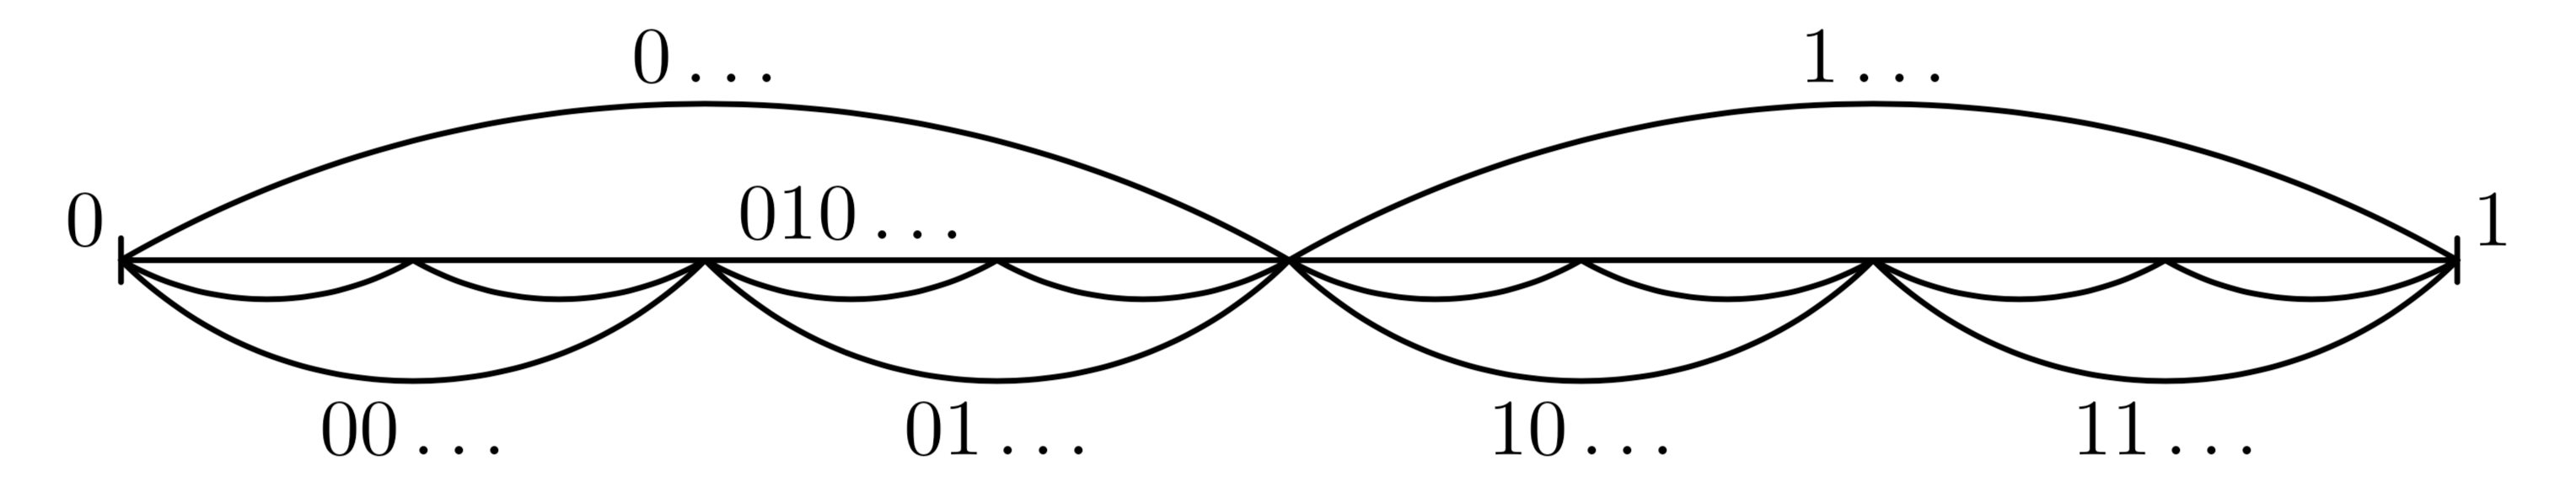
\includegraphics[width=0.6\textwidth]{binary}
\end{center}
Можно ли сказать, что мы тем самым построили взаимно однозначное соответствие между числами на отрезке $[0, 1]$ и бесконечными двоичными последовательностями (дробями)? Не совсем. Проблема в том, что это соответствие не взаимно однозначно, некоторым числам соответствуют две последовательности. А именно, это происходит, когда точка попадает на границу очередного отрезка. Тогда мы можем относить её как к левой, так и к правой половине. В результате, например, последовательности $0,1001111...$ и $0,101000...$ соответствуют одному и тому же числу.
\newline
Как же исправить положение? Мы получим взаимно однозначное соответствие, если исключим последовательности, в которых начиная с некоторого момента все цифры равны 1 (одну такую последовательность мы всё же должны оставить – это $0.111...$). Но таких последовательностей счётное множество, так что их добавление не меняет мощности множества по вышеприведенной лемме.
\end{proof}




\subsection{Теорема Кантора о неравномощности множества и множества его подмножеств.}
\begin{theorem}
Никакое множество X не равномощно множеству своих подмножеств.
\begin{proof}
Предположим, что множество $X$ и множество всех его подмножеств (оно обозначается $2^X$ ) равномощны. Пусть $f$ — биекция из $X$ в $2^X$ . Рассмотрим те элементы $x$, которые не принадлежат соответствующим им подмножествам, то есть $x \notin f(x)$. Рассмотрим теперь множество всех таких элементов:
\[
Y = \{x \in X | x \notin f(x)\}.
\]
До противоречия осталось совсем немного: оказывается, что этому множеству $Y$ не может соответствовать никакой элемент множества $X$. Действительно, пусть $Y = f(y)$ для некоторого $y \in X$. Тогда
\[
y \in Y
\Leftrightarrow
y \notin f(y)
\Leftrightarrow
y \notin Y,
\]
здесь первая равносильность верна по определению множества $Y$ , а вторая – поскольку $f (y) = Y$ . Мы получили противоречие, а значит такой биекции $f$ не существует.
\end{proof}
\end{theorem}






\subsection{Теорема Кантора—Бернштейна.}
\begin{theorem}
Если для множеств $A$ и $B$ существует инъекция из $A$ в $B$ и инъекция из $B$ в $A$, то существует и биекция между $A$ и $B$.
\begin{proof}
Пусть $f : A \to B$ и $g : B \to A$ – инъекции. Рассмотрим (возможно, бесконечный) ориентированный граф с вершинами $A \cup B$ (для простоты обозначений предположим, что $A$ и $B$ не пересекаются). Для точек $x \in A$ и $y \in B$ мы проводим ребро из $x$ в $y$, если $f(x) = y$, и ребро из $y$ в $x$, если $g(y) = x$. Если нарисовать множество $A$ слева, а множество $B$ справа, то можно сказать, что мы проводим рёбра слева направо согласно функции $f$ и справа налево согласно функции $g$.
\newline
По построению из каждой точки выходит ровно одно ребро. А сколько рёбер входит? Поскольку функции инъективны, то не больше одного (но может не входить ни одного).
\newline
Разобьем граф на компоненты связности (забыв для этого об ориентации рёбер) и рассмотрим каждую компоненту отдельно. Как устроены эти компоненты? Есть три возможности. Связная компонента может быть
\begin{itemize}
    \item циклом из стрелок;
    \item бесконечной цепочкой стрелок, начинающейся в некоторой вершине (в которую ничего не входит);
    \item бесконечной в обе стороны цепочкой стрелок.
\end{itemize}
В самом деле, вперёд всегда можно идти по единственной стрелке, а назад либо можно пойти единственным образом, либо нельзя пойти вовсе. Если, идя вперёд, мы дважды попадём в одну вершину, то образуется цикл (и это возможно, лишь если мы вернёмся в начальную вершину). Если нет, то образуется бесконечная цепочка вперёд; её можно однозначно продолжать назад, при этом либо мы упрёмся в вершину, где назад не пройти, либо получим двустороннюю цепочку.
\newline
Это верно для любого ориентированного графа, в котором из каждой вершины выходит ровно одна стрелка и в каждую вершину входит не больше одной стрелки. В нашем конкретном случае есть дополнительная структура: вершины бывают левые и правые (из $A$ и из $B$). Они чередуются, поэтому цикл может быть только чётной длины и содержит поровну вершин из $A$ и из $B$. Любое из отображений $f$ и $g$ может быть использовано, чтобы построить биекцию между $A$- и $B$-вершинами цикла (так что есть минимум два варианта биекции). То же самое верно для бесконечной в обе стороны цепочки (два варианта). Если же цепочка бесконечна только в одну сторону, то для построения биекции годится только одно из отображений. Скажем, если она начинается с элемента $a \in A$, то годится только функция $f$ (при которой a соответствует $f(a)$, затем $g(f(a))$ соответствует $f(g(f(a)))$ и так далее). Но в любом случае одна из функций $f$ и $g$ годится, так что внутри каждой связной компоненты у нас есть биекция, и остаётся их объединить для всех связных компонент.
\end{proof}
\end{theorem}







\subsection{Формула Байеса. Формула полной вероятности.}
\begin{lemma}
\normalfont{(формула Байеса).} Если вероятность событий $A$ и $B$ положительна, то
\[
Pr[A | B] = Pr[A] \cdot \frac{Pr[B | A]}{Pr[B]}.
\]
\begin{proof}
Доказательство формулы Байеса почти очевидно. Достаточно просто записать вероятность события $A \cap B$ через условные вероятности двумя способами:
\[
Pr[A \cap B] = Pr[B] \cdot Pr[A | B] = Pr[A] \cdot Pr[B | A].
\]
Теперь второе равенство сразу даёт формулу Байеса.
\end{proof}
\end{lemma}
\begin{lemma}
Пусть $B_1,...,B_n$ -- разбиение вероятностного пространства U, то есть $U = B_1 \cup ... \cup B_n$, где $B_i \cap B_j = \varnothing$ при $i \neq j$. Пусть также $Pr[B_i] > 0$ для всякого $i$. Тогда для всякого события $A \subset U$
\[
Pr[A] = \sum_{i=1}^n Pr[A | B_i] \cdot Pr[B_i].
\]
\begin{proof}
Согласно свойству аддитивности вероятности
\[
Pr[A] = \sum_{i=1}^{n} Pr[A \cap B_i] = \sum_{i=1}^n Pr[A | B_i] \cdot Pr[B_i],
\]
где первое равенство получается по формуле сложения вероятностей непересекающихся событий, а второе равенство -- по определению условной вероятности.
\end{proof}
\end{lemma}




\subsection{Парадокс дней рождений (математическое ожидание числа людей с совпавшими днями рождений).}
Рассмотрим $n$ случайных людей и посмотрим на количество совпадений дней рождения у них, то есть на количество пар людей, имеющих день рождения в один день. Каким в среднем будет это число?
\newline
Сформулируем вопрос точно. Вероятностное пространство: всюду определённая функция из $n$-элементного множества людей $\{x_1, ..., x_n\}$ в 365-элементное множество дней в году. Все исходы равновозможные.
\newline
Обозначим случайную величину, равную количеству пар людей с совпадающими днями рождения, через $f$. Нам требуется посчитать математическое ожидание случайной величины $f$. Но при этом случайная величина довольно сложная, и подсчитывать математическое ожидание непосредственно из определения трудно.
\newline
Идея состоит в следующем: давайте разобьём сложную случайную величину $f$ в сумму нескольких простых случайных величин. Тогда мы сможем подсчитать отдельно математические ожидания всех простых величин, а затем, пользуясь линейностью математического ожидания, просто сложить результаты.
\newline
Обозначим через $g_{ij}$ случайную величину, равную 1, если у людей $x_i$ и $x_j$ дни рождения совпадают, и равную 0 в противном случае. Тогда можно заметить, что
\[
f = \sum_{i < j} g_{ij}.
\]
Подсчитаем математическое ожидание случайной величины $g_{ij}$. Нетрудно увидеть, что вероятность того, что у двух случайных людей дни рождения совпадают, равна $1/365$, так что с вероятностью $1/365$ случайная величина равна 1, и с вероятностью $1-1/365$ равна 0. Так что $E[g_{ij}] = 1/365$ (для всякой пары $i,j$). Для математического ожидания $f$ из линейности получаем
\[
E[f] = E[\sum_{i<j} g_{ij}] = \sum_{i<j} E[g_{ij}] = 
\sum_{i<j} 1/365 = \frac{n(n-1)}{2 \cdot 365}.
\]
Например, если число людей $n$ больше 27, то $E[f] > 1$, то есть естественно ожидать, что будет не меньше одного совпадения дней рождений, что может показаться противоречащим интуиции (поэтому эту задачу иногда называют «парадоксом дней рождения»).



\subsection{Неравенство Маркова.}
\begin{lemma}
Пусть $f$ — случайная величина, принимающая
только неотрицательные значения. Тогда для всякого $\alpha > 0$ верно
\[
Pr[f \geqslant \alpha] \leqslant
\frac{E[f]}{\alpha}
\]
\begin{proof}
Взглянем на нужное нам неравенство с другой стороны. Нам нужно доказать, что
\[
E[f] \geqslant \alpha \cdot Pr[f \geqslant \alpha]
\]
Пусть случайная величина $f$ принимает значения $a_1, ..., a_k$ с вероятностями $p_1,...,p_k$. Запишем, чему равно её математическое ожидание по определению:
\[
E[f] = \alpha_1 p_1 + \alpha_2 p_2 + ... + \alpha_k p_k.
\]
Посмотрим отдельно на те $a_i$, которые меньше $\alpha$, и отдельно на те $a_i$, которые не меньше $\alpha$. Если первые заменить на ноль, то сумма может только уменьшиться. Если вторые заменить на $\alpha$, то сумма также может только уменьшиться. После таких замен, у нас остаётся сумма нескольких слагаемых, каждое из которых есть $\alpha p_i$, где $p_i$ — вероятность некоторого значения случайной величины, не меньшего $\alpha$. Нетрудно видеть, что такая сумма как раз равна $\alpha \cdot Pr[f \geqslant \alpha]$ и лемма доказана.
\end{proof}
\end{lemma}







\subsection{\textcolor{orange}{(UNCHECKED)} Нижняя оценка на числа Рамсея $R(k, k)$.}
\textit{Число $R(m,n)$ -- такое наименьшее число $x$, что при любой раскраске ребер полного графа $K_x$ в два цвета либо в нем найдется подграф $K_m$ с ребрами цвета 1,
либо в нем найдется подграф $K_n$ с ребрами цвета 2.}
\begin{theorem}[Эрдеша]
При $k \geqslant 2$ справедливо неравенство
\[
R(k,k) \geqslant 2^{k/2}.
\]
\begin{proof}
Рассмотрим $k \geqslant 3$, т.к. $R(2,2) = 2$. Оценим долю $\gamma (p,k)$ графов с $p$ помеченными вершинами, в которых найдется полный подграф с $k$ вершинами.
Возможных ребер в графах с $p$ вершинами ровно $\binom{p}{2}$, откуда графов с $p$ вершинами в точности $2^{\binom{p}{2}}$.
Выбрать $k$ вершин, образующих полный подграф, из $p$ вершин можно $\binom{p}{k}$ способами. Оставшиеся $\binom{p}{2} - \binom{k}{2}$ могут быть проведены произвольно. Поэтому число графов с $p$ вершинами, содержащих полный подграф с $k$ вершинами, не более $\binom{p}{k} \cdot 2^{\binom{p}{2} - \binom{k}{2}}$. Значит,
\[
\gamma(p,k) \leqslant \frac{\binom{p}{k} \cdot 2^{\binom{p}{2} - \binom{k}{2}}}{2^{\binom{p}{2}}} = \frac{p^k}{k!2^{\binom{k}{2}}}
\]
При $p < 2^{k/2}$ получаем
\[
\gamma (p,k) < \frac{2^{k^2/2}}{k! 2^{k^2/2 - k/2}} =
\frac{2^{k/2}}{k!} < \frac{1}{2}
\]
Разобьем все графы с $p$ вершинами на пары $(G, \overline{G})$.
Тогда по доказанному выше при $p < 2^{k/2}$ в этом разбиении найдется такая пара графов $(G, \overline{G})$, что ни $G$, ни $\overline{G}$ не содержат полный подграф с $k$ вершинами.
Поэтому $R(k,k) \geqslant 2^{k/2}$.
\end{proof}
\end{theorem}











\subsection{Нижняя оценка на максимальное количество ребер в разрезе.}
Рассмотрим простой неориентированный граф $G = (V,E)$. Разрезом графа называется разбиение множества его вершин на два непересекающихся подмножества: $V_1 \cup V_2, V_1 \cap V_2 = \varnothing$. Мы говорим, что ребро попадает в разрез, если один его конец лежит в $V_1$, а другой в $V_2$. Размером разреза называется число рёбер, попадающих в разрез. Нас будут интересовать большие разрезы графа.
\begin{theorem}
Всякий граф $G = (V, E)$ имеет разрез размера не меньше $|E|/2$.
\begin{proof}
Рассмотрим случайный разрез графа $G$. Более точно, мы берем равномерное распределение на множестве всех разрезов. Разрез задается подмножеством $S \subset V$: такому подмножеству ставится в соответствие разрез $(S, V \setminus S)$. Всего подмножеств (а значит и разрезов) $2^n$, так что вероятность каждого разреза есть $1/2^n$. Можно проверить, что для каждой пары вершин $x \neq y$ все четыре события <<$x \in S, y \in S$>>, <<$x \notin S, y \in S$>>, <<$x \in S, y \notin S$>>, <<$x \notin S, y \notin S$>> имеют вероятность $1/4$.
Итак, рассмотрим случайный разрез и рассмотрим случайную величину $f$, равную размеру разреза. Посчитаем ее математическое ожидание. Для этого, как и раньше, стоит разбить случайную величину в сумму более простых случайных величин. Для всякого $e \in E$ рассмотрим случайную величину $f_e$, равную 1, если ребро  $e$ входит в разрез, и равную 0 в противном случае. Тогда нетрудно видеть, что $f = \sum_{e \in E} f_e$, а значит
\[
E[f] = \sum_{e \in E} E[f_e].
\]
Однако, для случайной величины $f_e$ математическое ожидание уже нетрудно посчитать. Действительно, для всякого фиксированного ребра $e$ вероятность, что оно попадет в разрез равна $1/2$. А значит, $E[f_e] = 1/2$ для всякого $e \in E$, откуда
\[
E[f] = \sum_{e \in E} 1/2 = |E|/2.
\]
Из этого следует, что есть конкретный разрез, содержащий не меньше $|E|/2$ ребер.
\end{proof}
\end{theorem}
















\subsection{Существование и единственность полинома Жегалкина (в стандартном виде) для любой булевой функции.}
\begin{theorem}
Всякая булева функция единственным образом представляется в виде полинома Жегалкина.
\begin{proof}
Заметим, что различных булевых функций от $n$ переменных $2^{2^n}$ штук. При этом конъюнкций вида $x_{i_1}...x_{i_k}$ существует ровно $2^n$, так как из $n$ возможных сомножителей каждый или входит в конъюнкцию, или нет. В полиноме у каждой такой конъюнкции стоит 0 или 1, то есть существует $2^{2^n}$ различных полиномов Жегалкина от $n$ переменных.
\newline
\newline
Теперь достаточно лишь доказать, что различные полиномы реализуют различные функции. Предположим противное. Тогда приравняв два различных полинома и перенеся один из них в другую часть равенства, получим полином, тождественно равный нулю и имеющий ненулевые коэффициенты. Тогда рассмотрим слагаемое с единичным коэффициентом наименьшей длины, то есть с наименьшим числом переменных, входящих в него (любой один, если таких несколько). Подставив единицы на места этих переменных, и нули на места остальных, получим, что на этом наборе только одно это слагаемое принимает единичное значение, то есть нулевая функция на одном из наборов принимает значение 1. Противоречие. Значит, каждая булева функция реализуется полиномом Жегалкина единственным образом.
\end{proof}
\end{theorem}



\subsection{Существование булевых функций от n переменных схемной сложности больше $(c2^n)/n$.}
\begin{lemma}
Для всякого $n \geqslant 10$ существует функция $ f : \{0, 1\}^n \to \{0, 1\}$, которую нельзя вычислить схемой размера меньше $2^n/10n$.
\begin{proof}
Для доказательства применим мощностной метод: докажем, что функций больше, чем маленьких схем. Тогда маленьких схем не хватит, чтобы вычислить все функции.
\newline
Всего булевых функций от $n$ переменных $2^{2^n}$.
\newline
Заметим, что если схемная сложность функции не больше $S$, то существует схема размера ровно $S$, вычисляющая эту функцию (добавим в схему столько присваиваний $x_1 \wedge x_1$, сколько нужно для выравнивания размера).
\newline
Оценим (весьма грубо, но для наших целей такой оценки будет достаточно) количество схем размера $S$ от $n$ переменных. Для этого заметим, что всякую схему размера $S$ с $n$ переменными можно описать с помощью не больше чем $S \cdot 2(1+\log(n+S))$ битов. Для описания схемы удобно её расширить, добавив в начало все переменные.
\newline
Теперь для каждого из $S$ элементов схемы нужно указать его тип (конъюнкция, дизъюнкция, отрицание), на что достаточно потратить два бита. Кроме того, нужно указать, к каким из предыдущих элементов применяется операция. Достаточно указать номера элементов в расширенной последовательности, начинающейся со всех переменных схемы. На это требуется не более $S·2(1+\log(n+S))$ битов.
\newline
Мы применим эту оценку на длину описания схемы при $S = \lceil 2^n/10n \rfloor$. В этом случае, как легко проверить, $S > n$ при $n \geqslant 10$. Оценка на длину описания упрощается:
\[
S \cdot 2(1 + \log(n + S)) \geqslant 2S \cdot (2 + \log_2{S})
\geqslant 4S \log{S}.
\]
Таким образом, при $n \geqslant 10$ и $S = \lfloor 2^n/10n \rfloor$ всякую схему размера $S$ можно описать строкой из не более \(
4 \frac{2^n}{10n} (n - \log_2{10n})
\geqslant
2 \cdot 2^n / 5
\) битов. Поэтому количество схем размера $S$ не больше, чем количество таких строк, то есть не больше $2^{2 \cdot 2^n / 5}$. Видно, что это меньше $2^{2^n}$, а значит не всякую функцию можно вычислить схемой размера $S$ (или меньшего, как мы заметили с самого начала).
\end{proof}
\end{lemma}









\subsection{Верхняя оценка $O(n2^n)$ схемной сложности булевой функции от n переменных.}
\begin{lemma}
Всякую функцию $f : \{0, 1\}^n \to \{0, 1\}$ можно вычислить схемой размера не больше $O(n2^n)$.
\begin{proof}
Для всякого $a \in \{0, 1\}^n$ рассмотрим такую функцию $f_a : \{0, 1\}^n \to \{0, 1\}$, что $f (x) = 1$ тогда и только тогда, когда $x = a$. Будет удобно ввести обозначения $x^1 = x$ и $x^0 = \neg x$. Тогда функцию $f_a$ можно записать формулой
\[
f_a(x) = \bigwedge_{i=1}^n x_i^{a_i},
\]
где $x = (x_1,...,x_n)$ и $a = (a_1,...,a_n)$.
\newline
Произвольная функция $f$ выражается через функции $f_a$ с помощью дизъюнкции:
\[
f(x) = \bigvee_{a \in f^{-1}(1)} f_a(x).
\]
Эти формулы без труда переделываются в схему. Наша схема сначала будет вычислять отрицания всех переменных, на это нужно $n$ элементов. После этого можно вычислить все функции $f_a$. Для вычисления каждой такой функции нужно $n-1$ раз применить конъюнкцию. Всего получается $2^n(n-1)$ элемент. Наконец, для вычисления $f$ нужно взять дизъюнкцию нужных функций $f_a$, на это уйдёт не более $2^n$ элементов. Суммарно в нашей схеме получается $O(n2^n)$ элементов.
\end{proof}
\end{lemma}










\subsection{\textcolor{orange}{(UNCHECKED)} Булевы схемы для сложения и умножения $n$-битовых чисел. Оценка размера.}
\begin{wrapfigure}{r}{0.4\textwidth}
    \centering
    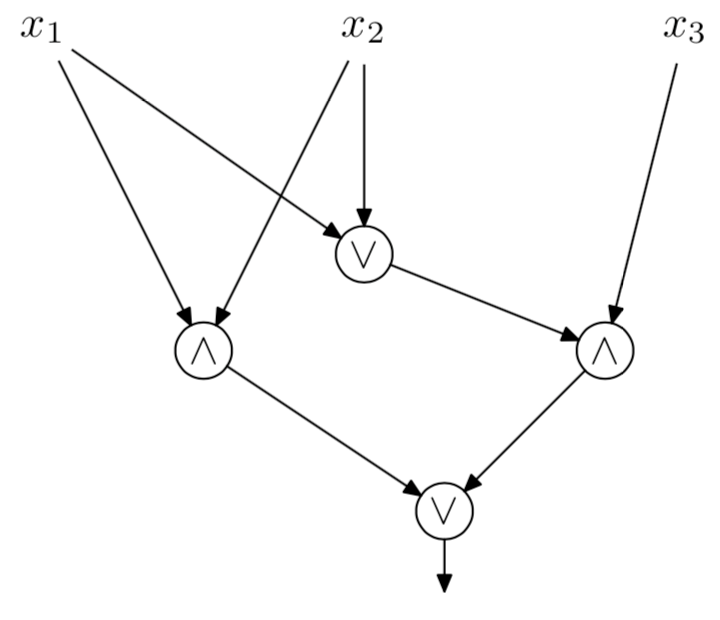
\includegraphics[width=0.25\textwidth]{maj}
    \caption{Схема для функции $MAJ_3$}
\end{wrapfigure}
Пусть нам даны две $n$-битовых двоичных записи чисел $x$ и $y$ и мы хотим вычислить двоичную запись их суммы $z = x + y$. Для удобства обозначим $x = x_{n-1} ... x_1x_0$, где $x_0$ -- младший разряд двоичной записи. Аналогично, $y = y_{n-1} ... y_1y_0$. Во-первых, заметим, что в двоичной записи $z$ будет не более $n + 1$ разрядов. Так что мы хотим построить схему с $2n$ входами и $n + 1$ выходом.
\newline
Идея конструкции схемы будет та же, что и в обычном школьном сложении в столбик. Мы будем складывать числа $x$ и $y$ поразрядно, попутно вычисляя биты переноса в следующий разряд.
\newline
Для удобства будем обозначать через $b_i$ бит, который переносится в $i$-ый разряд из предыдущих.
\newline
Заметим, что мы уже готовы вычислить первый разряд ответа $z_0 = x_0 \oplus y_0$. Далее, заметим, что $b_1 = x_0 \wedge y_0$, добавим соответствующий элемент в схему. Перейдём к следующему разряду. Здесь $z_1 = x_1 \oplus y_1 \oplus b_1$ и $b_2 = MAJ_3(x_1,y_1,b_1)$. Для вычисления первого добавим сначала подсхему, вычисляющую промежуточную величину $c_1 = x_1 \oplus y_1$, а затем подсхему, вычисляющую $z_1 = c_1 \oplus b_1$. Для вычисления $b_2$ просто добавим подсхему, вычисляющую функцию $MAJ_3$. Такая схема также приведена выше. Дальше, случай произвольных $z_i$ и $b_i$ полностью аналогичен случаю $z_1$ и $b_1$ и мы можем последовательно вычислить все эти значения.
\newline
Оценим теперь размер описанной схемы. Для каждого разряда ответа нам нужно не больше двух раз применить подсхему для вычисления функции $\oplus$ и не более одного раза подсхему для вычисления $MAJ_3$. Все эти схемы имеют фиксированный размер, так что для вычисления каждого разряда $z$ мы используем фиксированное число элементов, не зависящее от числа входных переменных. Поэтому всего в схеме $O(n)$ элементов.
\begin{center}
    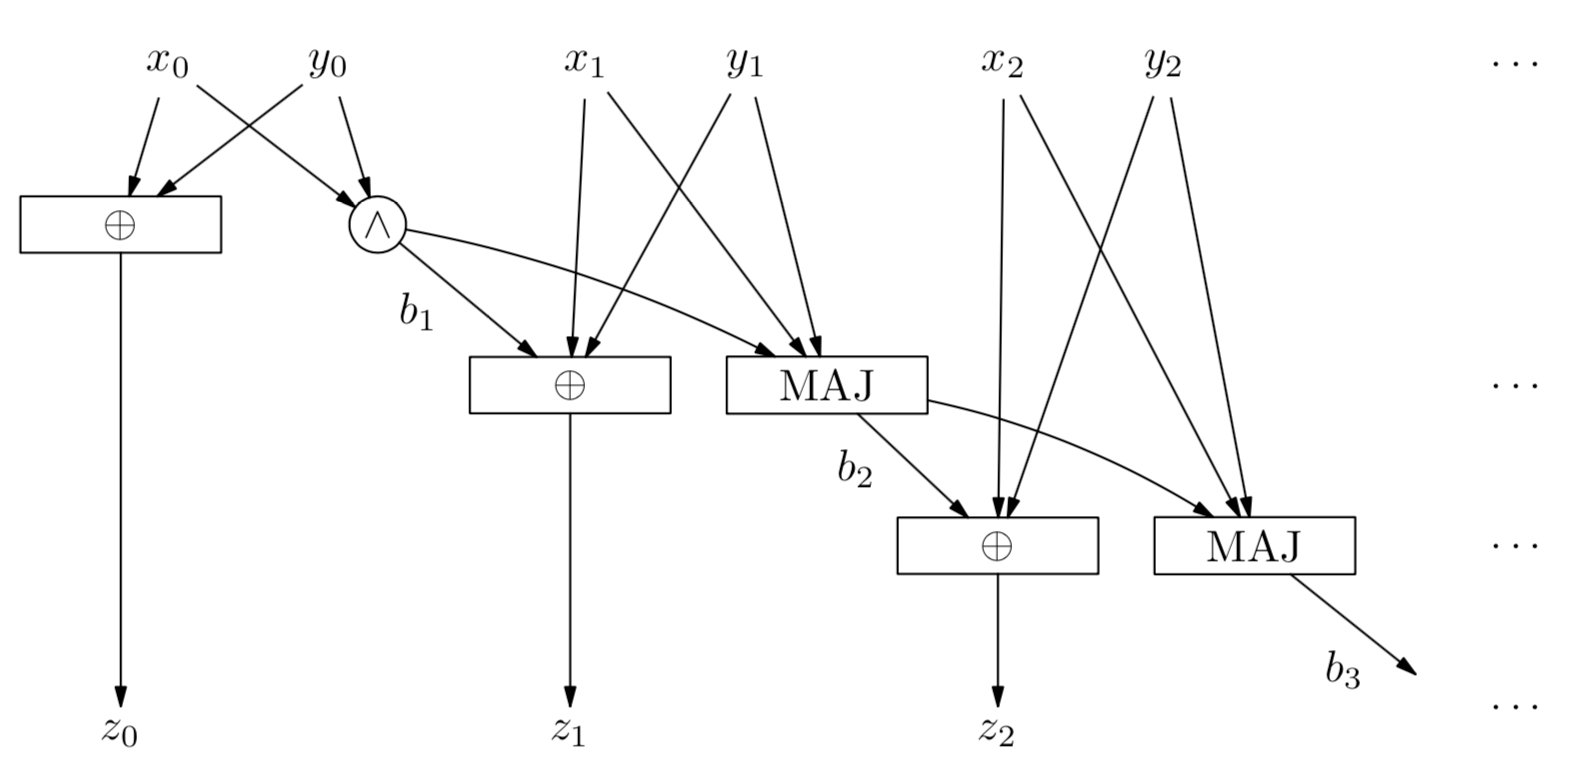
\includegraphics[width=0.5\textwidth]{sum}
\end{center}
Построим теперь схему для умножения $n$-битовых чисел. Пусть на вход снова подаются два числа $x = x_{n-1} ...x_1x_0$ и $y = y_{n-1} ...y_1y_0$. На этот раз мы хотим вычислить $z = x \cdot y$. Заметим, что $z$ имеет не больше $2^n$ разрядов. Действительно, $x,y < 2^n$, так что $z = x \cdot y < 2^{2n}$, а значит для его записи достаточно $2n$ разрядов.
\newline
Для вычисления $z$ снова воспользуемся школьным методом. В нем умножение двух чисел сводится к сложению $n$ чисел. Действительно, чтобы умножить $x$ на $y$ достаточно для всякого $i = 0, ... , n - 1$ умножить $x$ на $y_i$, приписать в конце числа $i$ нулей и затем сложить все полученные числа.
\newline
Умножение $x$ на $y_i$ легко реализуется с помощью $n$ конъюнкций. Чтобы приписывать нули, их нужно иметь. В нашем определении не разрешается использовать константы. Поэтому нуль нужно вычислить. Для этого годится, например, такая схема
\[
\neg x_1, x_1 \wedge \neg x_1 = 0
\]
После этого остается сложить $n$ чисел длины не более $2n$. Для этого мы можем $n-1$ раз применить схему для сложения, описанную выше. Размер каждой схемы для сложения линейный, так что суммарная сложность схемы для умножения получается $O(n^2)$.



\subsection{Булева схема для задачи о связности графа. Оценка размера.}
Во-первых, стоит обсудить, как задавать граф в пригодном для схем виде. Для этого удобно воспользоваться так называемой матрицей смежности графа. Перенумеруем вершины графа $v_1, v_2, ... , v_n$. Матрицей смежности графа $G$ называется матрица $A \in \{0,1\}^{n \times n}$, в которой на пересечении строки $i$ со столбцом $j$ стоит 1 тогда и только тогда, когда в графе есть ребро $vi - vj$.
\newline
Матрица смежности полностью описывает, какие пары вершин соединены рёбрами, так что булевой схеме достаточно подать на вход матрицу смежности графа. Более того, заметим, что матрица смежности симметрична и на диагонали у неё обязательно стоят нули (мы запрещали петли — рёбра, ведущие из вершины в неё же саму). Так что на вход схеме можно подать, скажем, только верхнюю половину матрицы смежности.
\newline
Оказывается, матрица смежности также удобна для проверки связности графа. Можно матрицу $A$ интерпретировать следующим образом: на пересечении строки $i$ и столбца $j$ написано количество путей длины 1 из вершины $v_i$ в вершину $v_j$ . Теперь возведём матрицу $A$ в квадрат (над действительными числами). Если посмотреть на формулу для произведения матриц можно заметить, что на пересечении строки $i$ и столбца $j$ матрицы $A^2$ записано количество путей длины 2 из вершины $v_i$ в вершину $v_j$. По индукции можно доказать, что на пересечении строки $i$ и столбца $j$ матрицы $A^k$ записано число путей длины $k$ из вершины $v_i$ в вершину $v_j$ . Заметим теперь, что если между какими-то двумя вершинами в графе есть путь, то обязательно есть путь длины не больше $n - 1$ (из пути всегда можно выкинуть циклы, если они там есть, после этого все вершины в пути разные). Так что для проверки связности у нас появляется такой план: вычислим все матрицы $A,A^2,...,A^{n-1}$ и для каждой пары вершин $v_i$ и $v_j$ проверим, есть ли между ними путь длины не больше $n - 1$. Если это так, то граф связен, иначе не связен.
\newline
Этот план можно несколько упростить. Во-первых, можно немного модифицировать матрицу смежности. Рассмотрим матрицу $A'$, которая отличается от матрицы $A$ тем, что у неё на главной диагонали стоят единицы, а не нули (в остальном матрицы совпадают). В терминах графов это означает, что к каждой вершине мы добавляем петлю. В модели простых неориентированных графов мы этого не допускали, но ничего не мешает нам рассмотреть графы с петлями. Идея состоит в том, что теперь, если между двумя вершинами есть путь длины меньше $n-1$, то есть и путь длины ровно $n - 1$ (достаточно добавить к пути нужное количество петель). Так что теперь не обязательно смотреть на все степени матрицы смежности, достаточно взглянуть на $(A')^{n-1}$. Если в ячейках этой матрицы нет нулей, то граф связен, иначе не связен.
\newline
Второе упрощение связано со способом возведения матрицы в степень. Выше мы считали число путей и для этого нужно складывать и умножать целые числа. Чтобы делать это с помощью булевых схем, нам придётся использовать описанные выше схемы для сложения и умножения. Чтобы оценить размер получившейся схемы, придётся оценивать величину возникающих в процессе вычислений целых чисел. От этих сложностей можно избавиться.
\newline
Решение состоит в том, чтобы вместо умножения матриц над целыми числами воспользоваться так называемым \textit{булевым умножением матриц}. В нем формулы для умножения матриц такие же, как и в обычном умножении, только вместо операции умножения используется конъюнкция, а вместо сложения – дизъюнкция. Тогда по индукции можно доказать, что в (булевой) матрице $(A')^k$ на пересечении строки $i$ и столбца $j$ стоит 1 тогда и только тогда, когда в графе есть путь из $v_i$ в $v_j$ длины не больше $k$.
\newline
Теперь мы готовы описать схему для проверки графа на связность. На вход схема (по существу) получает матрицу смежности $A'$. Схема последовательно вычисляет булевы степени этой матрицы $(A')^2, . . . , (A')^{n-1}$. Затем схема вычисляет конъюнкцию всех ячеек матрицы $(A')^{n-1}$ и подаёт её на выход.
\newline
Оценим размер получившийся схемы. Для булева умножения двух булевых матриц $n \times n$ достаточно $n^2 \cdot O(n) = O(n^3)$ операций (каждая ячейка произведения матриц вычисляется за линейное число операций, всего ячеек $n^2$). Всего нам нужно $(n-1)$ умножение матриц, так что для вычисления матрицы $(A')^{n-1}$ достаточно $O(n^4)$ операций. На последний этап (конъюнкция ячеек $(A')^{n-1}$) нужно $O(n^2)$ операций, итого получается $O(n^4) + O(n^2) = O(n^4)$ операций.









\subsection{Задача об угадывании числа. Верхняя и нижняя оценки.}
\begin{lemma}
Для угадывания числа от 1 до $N$ необходимо и достаточно $\lceil \log_2{N} \rceil$ вопросов.
\end{lemma}
Рассмотрим следующую игру. Алиса загадывает натуральное число от 1 до $N$, а Боб пытается это число отгадать. При этом Бобу разрешается задавать вопросы, на которые Алиса может ответить “да” или “нет”, и Алиса должна на эти вопросы давать правильные ответы. Цель Боба состоит в том, чтобы задать как можно меньше вопросов. При этом мы не хотим полагаться на удачу, то есть нужно, чтобы число вопросов было гарантировано небольшим. Другими словами, мы хотим найти такое минимальное $k$, что у Боба есть алгоритм, позволяющий отгадать число за не более чем $k$ вопросов, какое бы число ни загадала Алиса.
\newline
Оказывается, что Бобу всегда достаточно задать не более чем $\lceil \log_2{N} \rceil$ вопросов. Чтобы это доказать мы воспользуемся \textit{методом деления пополам}. Идея в том, что Боб каждым своим вопросом будет сокращать количество оставшихся возможных чисел примерно в два раза. Этого можно добиться, например, так. Обозначим число, загаданное Алисой, через $x$. На каждом шаге Боб будет знать, что $x$ лежит в некотором “отрезке” $\{y | a \leqslant y \leqslant b\}$ для каких-то $a$ и $b$.Изначально $a=1$ и $b=N$. На очередном шаге Боб будет вычислять $c = \lfloor (a + b)/2 \rfloor$ и спрашивать, верно ли, что $x \leqslant c$ Если Алиса отвечает “да”, то Боб переходит к отрезку $\{y | a \leqslant y \leqslant c\}$ и повторяет процедуру. Иначе, Боб переходит к отрезку $\{y | c+1 \leqslant y \leqslant b\}$и также повторяет процедуру. Нетрудно видеть, что каждый раз длина отрезка уменьшается почти в два раза (если в отрезке было нечетное число точек, то в следующем отрезке может оказаться чуть больше чем половина точек). Так что через приблизительно $log_2 N$ шагов в отрезке останется одна точка и Боб узнает число Алисы. На самом деле, нетрудно доказать, что достаточно $\lceil log_2 N \rceil$ вопросов, что мы сейчас и сделаем.
\newline
Оказывается, что доказанная только что оценка точная: не существует алгоритма, который для всякого загаданного Алисой числа задавал бы меньше $\lceil log_2 N \rceil$ вопросов. Сейчас мы докажем эту нижнюю оценку сложности нашей задачи.
\newline
Для доказательства нижней оценки мы применим так называемый мощностной метод. Пусть у Боба есть какой-то алгоритм сложности $k$ (то есть, в нем всегда задается не более $k$ вопросов), Алиса загадала какое-то число и Боб задал свои вопросы. Рассмотрим цепочку ответов Алисы. Для удобства будем обозначать ответ “да” цифрой 1, а ответ “нет” цифрой 0. Тогда последовательность ответов Алисы – это последовательность из 0 и 1 длины не больше $k$. Заметим, что для двух разных загаданных Алисой чисел последовательности не могут совпадать. Действительно, если для двух различных $x$ и $y$ Алиса дает Бобу на его вопросы полностью одинаковые ответы, то для Боба эти случаи неразличимы: его диалоги с Алисой для $x$ и для $y$ выглядят одинаково. При этом Боб после этого диалога выдает какой-то ответ, который определяется только состоявшимся диалогом. Значит в одном из случаев его ответ будет неправильным. Далее, заметим, что не может быть так, что для двух различных $x$ и $y$, загаданных Алисой, цепочка ответов для $x$ является началом цепочки ответов для $y$. Действительно, иначе диалог Боба с Алисой выглядит одинаково для $x$ и $y$ до того момента, когда будут заданы все вопросы из цепочки ответов для $x$. Значит к этому моменту Боб не может отличить $x$ от $y$ и должен делать для них одно и то же, тогда как он в одном случае задает следующий вопрос, а в другом нет.
\newline
Таким образом, мы получили, что каждому числу от 1 до $N$ соответствует последовательность из не более чем $k$ нулей и единиц, все эти последовательности различны, и ни одна не является началом другой. Заметим, что семейство этих последовательностей содержит не более $2^k$ элементов. Действительно, если какая-то из них имеет длину меньше $k$, то продолжим ее, например, нулями. Тогда для различных $x$ и $y$ полученные последовательности длины $k$ различны: иначе они либо совпадают, либо одна (более короткая) является началом другой. Таким образом, каждому числу от 1 до $N$ соответствует последовательность длины $k$ из нулей и единиц, и все эти последовательности различны. Всего последовательностей длины $k$ из нулей и единиц $2^k$. По принципу Дирихле, чисел от 1 до $N$ должно быть не больше $2^k$ (иначе двум разным числам соответствуют одинаковые последовательности). Значит $N \leqslant 2^k$ то есть $k \geqslant log_2 N$ Поскольку $k$–целое число, то отсюда следует, что $k \geqslant \lceil log_2 N \rceil$.










\subsection{Задача о сортировке нижняя оценка.}
Дано $n$ объектов, все разного веса. За один шаг разрешается сравнить веса двух объектов (мы узнаем, какой из этих объектов тяжелее). Требуется расположить эти объекты в порядке возрастания веса.
\newline
Опишем теперь задачу формально. Удобно считать, что объекты изначально расположены в виде последовательности. Обозначим в этой последовательности самый тяжелый объект единицей, второй по тяжести -- двойкой, и так далее, самый легкий объект обозначим $n$. Таким образом, нам на вход по существу подается перестановка $n$-элементного множества. Чтобы упорядочить объекты по возрастанию нам нужно найти данную перестановку. Таким образом, в этом примере $A$ -- множество перестановок $n$-элементного множества и требуется вычислить тождественную функцию на $A$, то есть $f(x) = x$ для всякого $x \in A$.
\newline
При этом нам разрешается задавать не любые вопросы, а только вопросы о сравнении двух элементов перестановки. Формально это означает, что в вершинах разрешающего дерева могут стоять не любые подмножества множества перестановок, а только множества $S_{i,j}$ для $i, j = 1, ... , n$, состоящие из всех перестановок $(a_1, . . . , a_n)$, в которых $a_i > a_j$.
\begin{lemma}
Сложность задачи о сортировке $n$ объектов не меньше $\lceil \log_2{n!} \rceil$.
\begin{proof}
Заметим, что если бы не было ограничения на вид множеств, то задача была бы полностью аналогична задаче об угадывании числа: на вход подается один из $n!$ объектов и требуется угадать, какой именно. Поскольку у нас добавляется ограничение на тип вопросов, то наша задача усложняется, а значит в задаче о сортировке требуется не меньше вопросов.
\end{proof}
\end{lemma}









\subsection{Задача о нахождении самой тяжелой монеты. Верхние и нижние оценки.}
\begin{lemma}
Для нахождения самого тяжелого из $n$ объектов необходимо и достаточно $n - 1$ взвешивания.
\begin{proof}
Сначала докажем, что $n-1$ взвешивания достаточно. Проще всего вести рассуждение по индукции. Если $n = 1$, то ничего взвешивать не нужно. Пусть мы доказали утверждение для $n - 1$. Рассмотрим $n$ объектов. Возьмем любые два и сравним их. Заметим, что более легкий из них не может быть самым тяжелым, так что его можно выбросить из рассмотрения. Таким образом у нас остается $n - 1$ объект и по предположению индукции мы можем найти самый тяжелый из них за $n - 2$ оставшихся взвешивания.
\newline
Теперь докажем, что меньше чем за $n - 1$ взвешивание найти самый тяжелый объект нельзя. Пусть мы сделали $n - 2$ взвешивания. Рассмотрим следующий граф. Его вершинами будут наши объекты, и мы соединяем ребрами те из них, которые мы сравнили в одном из взвешиваний. Тогда в этом графе $n$ вершин и $n - 2$ ребра. Значит этот граф не связен. Рассмотрим множество $V_1$ объектов в одной из его компонент связности и множество $V_2$ всех остальных объектов. Предположим, для определенности, что самый тяжелый объект находится в $V_1$. Увеличим вес всех объектов в $V_2$ на одно и то же очень большое число, такое чтобы все объекты в $V_2$ стали тяжелее всех объектов в $V_1$. При этом результаты всех взвешиваний не изменятся, поскольку все сравнения были либо внутри $V_1$, либо внутри $V_2$, а самая тяжелая монета станет другой (теперь она будет в $V_2$). Таким образом, все взвешивания дадут один и тот же результат в обеих ситуациях, а самый тяжелый объект будет разным. Значит в одной из двух ситуаций наш протокол выдает неправильный ответ. Мы пришли к противоречию, а значит для нахождения самого тяжелого объекта требуется не меньше $n-1$ сравнения.


\end{proof}
\end{lemma}

\end{document}

